% Change 'digital' to 'printed' before printing
\documentclass[
  digital, %% This option enables the~default options for the
           %% digital version of a document. Replace with `printed`
           %% to enable the~default options for the~printed version
           %% of a document.
  table,   %% Causes the~coloring of tables. Replace with `notable`
           %% to restore plain tables.
  lof,     %% Prints the~List of Figures. Replace with `nolof` to
           %% hide the~List of Figures.
  lot,     %% Prints the~List of Tables. Replace with `nolot` to
           %% hide the~List of Tables.
  oneside,
  %% More options are listed in the~user guide at
  %% <http://mirrors.ctan.org/macros/latex/contrib/fithesis/guide/mu/fi.pdf>.
]{fithesis3}
%% The following section sets up the~locales used in the~thesis.
\usepackage[resetfonts]{cmap} %% We need to load the~T2A font encoding
\usepackage[main=english, slovak]{babel}

%% For non-Latin scripts, it may be necessary to load additional 
%% fonts:
\usepackage{paratype}
%%1
%% The following section sets up the~metadata of the~thesis.
\thesissetup{
    date          = 2017/5/22,
    university    = mu,
    faculty       = fi,
    type          = mgr,
    author        = Zuzana Dankovčíková,
    gender        = f,
    advisor       = Bruno Rossi PhD,
    title         = {Custom Roslyn Tool for Static Code Analysis},
    TeXtitle      = {Custom Roslyn Tool for Static Code Analysis},
    keywords      = {roslyn, C\#, compilers, code review, .NET compiler platform, Kentico, analyzer, code fix...},
    TeXkeywords   = {roslyn, C\#, compilers, code review, .NET compiler platform, Kentico, analyzer, code fix..., \ldots},
}
\thesislong{abstract}{
    TODO: This is the~abstract ...
}
\thesislong{thanks}{
    TODO: This is the~acknowledgement\dots

}

%% The following section sets up the~bibliography.
\usepackage{csquotes}
\usepackage[              %% When typesetting the~bibliography, the
  backend=biber,          %% `numeric` style will be used for the
  style=numeric,          %% entries and the~`numeric-comp` style
  citestyle=numeric-comp, %% for the~references to the~entries. The
  sorting=none,           %% entries will be sorted in cite order.
  sortlocale=auto         %% For more unformation about the~available
]{biblatex}               %% `style`s and `citestyles`, see:
%% <http://mirrors.ctan.org/macros/latex/contrib/biblatex/doc/biblatex.pdf>.
\addbibresource{mybib.bib} %% The bibliograpic database within
                          %% the~file `example.bib` will be used.

\usepackage{makeidx}      %% The `makeidx` package contains
\makeindex                %% helper commands for index typesetting.

%% These additional packages are used within the~document:
\usepackage{multirow}
\usepackage{paralist}
\usepackage{amsmath}
\usepackage{amsthm}
\usepackage{amsfonts}
\usepackage{url}
\usepackage{menukeys}
\usepackage{tikz-qtree}

\begin{document}
% =================================================================
% ============================= CHAPTER 1 =========================
% =================================================================
\chapter{Introduction}
TODO...
%Ideas:
%
%What is code quality, why is it important, tool that support it.. compilers, diversion ... aaaand here comes Roslyn which provides compiler as a platform.  
%
% --- Compilers + Roslyn ---
%In~the~.NET world, the~compiler used~to~be a~black box that given the~file paths to~the~source text, produced an~executable. In~order~to do that, compiler has to collect large amount of~information about the~code it is processing. This knowledge, however, was unavailable to~anyone but the~compiler itself and it was immediately forgotten once the~translated output was produced~\cite{roslyn-overview-github}. 
%
%Why is this an~issue when for decades this black-boxes served us well? Programmers are increasingly becoming reliant~upon the~powerful integrated development environments (IDEs). Features like IntelliSense, intelligent rename, refactoring or~"Find all references" are key~to~developers' productivity; and~even more so in~an~enterprise-size systems. 
%
%This gave a~rise to~number of~tools that analyze the~code for common issues and are able to~suggest a~refactoring. The problem is that that such~tool needs to~parse the~code first in~order~to be~able~to~understand and~analyze it. As a result companies need to invest fair amount of resources to duplicate the~logic that the~.NET compiler already possesses. Not only is it possible that the~compiler and the~tool may disagree on some specific piece of code, but with every new version of C\# the~tool needs to be updated to handle new language features\cite{dot-net-development-using-the-compiler-api}.
%
%With roslyn.. etc. etc. .. API for analysis.. use in companies for custom analyzers... etc. etc....
% https://github.com/dotnet/roslyn/wiki/Roslyn Overview -- motivation
%Make sure to stress out that ".NET Compiler Platform" and "Roslyn" names will be used interchangably as it is in Roslyn Succinctly on page 11.

% --- KEntico ---
%Kentico Software is an~IT company based in Brno, developing an~all-in-one solution for web content management, e-commerce and online marketing using ASP.NET architecture. The leading product is Kentico CMS (Content Management System) that has been on the~market since 2004 with 11th version currently being developed. 
%
%Over the~course of almost 13 years, feature after feature was added to the~product and the~solution grew to an~enormous extend. To give an~overview, the~current version of Kentico CMS contains XY projects and YZ source files. A lot of knowledge was accumulated and many internal conventions and guidelines were set. Much of the~features like globalization were developed in-house first, only to be added as an~integral part of the~.NET framework itself a few years later to be added.
%
%The size of the~company grew to more than 80 developers working on the~same product. It became increasingly harder to share all the~knowledge about the~internal conventions and even when trying to keep the~track of them, one can always forget about something when writing the~code. It is the~role of the~code review to spot those inconsistencies and make sure they are fixed. However, with the~increasing complexity of the~project, the~main focus of the~reviewer is to inspect the~general architecture and analyze how the~new code influences the~other parts of the~system, in order not to break anything. The manual and often repetitive task of checking the~compliance with the~internal guidelines and correct use of the~API during the~code review became very tiresome and dragged the~focus of the~reviewer from the~higher perspective on the~code.
%
%With this size of a codebase, number of internal knowledge and a large development team, the~need for an~automated tool checking for compliance with the~internal guidelines arose. 

%This led to a need for an~automated tool that would take care of the~repetitive checks that needed to be done by the~reviewer. Tools such as ReSharper or StyleCop, mentioned in the~Chapter~\ref{chap:static-code-analysis}, are easily configurable to enforce the~code style (spacing and naming conventions) and suggest general code refactorings. However, if a company wants to go beyond the~general best practices and enforce the~internal knowledge and rules to be followed, they must either use some advanced features of the~available static code analysis tools, which are often insufficient, or develop something on their own. 
%
%In Kentico this need led to a creation of an~internal tool called \textit{BugHunter}. The BugHunter is a very simple console application that given the~file path to the~solution, performs set of checks and outputs the~results. The output gives short desctrption on each problem along with an~information on its location (source file and line number).
%
%However, this tool is very primitive and has many issues. Since the~aim of this thesis is to check for the~same rules that the~old version of BugHunter does, the~following sections elaborate on the~downsides of this console application.
% =================================================================
% ============================= CHAPTER 2 =========================
% =================================================================
\chapter{Compilers}
\label{chap:compilers}
As~per~\cite{dragon-book}, a compiler is a~program that can read a~program in a~\textit{source} language and~translate it into a~semantically equivalent program in~a~\textit{target} language while reporting any errors detected in~the~translation process. The compiler may sometimes rely on other programs. For example, \textit{preprocessor} is responsible for collecting the~source code to be fed to the~compiler by expanding shorthands (macros) into source language statements. 

The compilation process can be divided into two parts: \textit{analysis} and \textit{synthesis}; commonly referred to as \textit{front end} and \textit{back end} of the~compiler.

The purpose of the~analysis part is to break up the~source program into chunks and build up a~grammatical structure that it corresponds to, based on the~source language grammar. This structure is subsequently transformed into an~intermediate representation of the~source program. Along the~way, the~compiler collects information about the~program and stores it into a~data structure called \textit{symbol table}. If any errors in syntax or semantics are encountered, analysis part shall inform the~programmer about the~problem. Otherwise, both intermediate representation and symbol table are passed to the~synthesis part where they are used for the~construction of the~target program.

The two main steps of compilation process internally consist of different phases as shown in Figure~\ref{fig:compiler-phases}. Each phase transforms one representation of source language into another, and passes it to the~following phase while working with the~symbol table during the~process. In synthesis phase, an~optional machine-independent optimizations can take place and are done on the~top of intermediate representation. After target machine code is generated, additional machine-dependent code optimizations are performed.

\begin{figure}[h!]
		\centering
			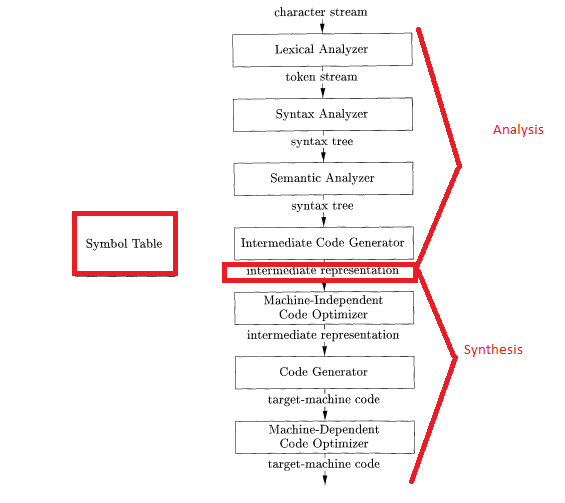
\includegraphics[scale=0.75]{img/compiler-phases}
		\caption{TODO: Phases of the~compiler~\cite{dragon-book}}
		\label{fig:compiler-phases}
\end{figure}

For the~purpose of this thesis, mainly the~analysis part is relevant and following section will elaborate on its respective phases.

  \section{Lexical analysis}
The compilation process starts with \textit{lexical analysis} or \textit{scanning}. The scanner transforms stream of characters of the~source program, as written by the~programmer, into the~series of meaningful sequences called \textit{lexemes}. Most programming languages allow for an~arbitrary number of white spaces to be present in the~source text to aid readability. However, white spaces, similarly as comments, are unimportant for the~target code generation itself, and thus the~lexical analyzer is responsible for discarding them completely.

In order to be able to correctly recognize the~lexeme, lexical analyzer may need to read ahead. For example, in C--like languages if the~scanner sees \texttt{<} character, it cannot decide whether it is a~lexeme for \textit{"less than"} operator or it is s part of \textit{"less then or equal to"} lexeme. In order to do that, it needs to read ahead and see if the~following character is \texttt{=} or not. Reading ahead is usually implemented with an~input buffer which the~lexical analyzer can read from and push back to. The use of buffer also boosts the~performance as fetching block of characters is more efficient as fetching one at a~time~\cite{dragon-book}.

The lexical analyzer typically uses regular expressions to identify the~lexemes and for each lexeme, it outputs a~\textit{token} (or \textit{token object}) of the~form 
\begin{equation}
  \langle token \textnormal{-} name, attribute \textnormal{-} name \rangle \textnormal{.}
\end{equation}

\noindent
For an~input sequence 
\begin{equation}
  total = 42 + base * interest
\end{equation}
 
the scanner output could be
\begin{equation}
  \langle id, 0 \rangle 
  \langle = \rangle 
  \langle num, 1 \rangle 
  \langle + \rangle 
  \langle id, 2 \rangle 
  \langle * \rangle 
  \langle id, 3 \rangle
\end{equation}

Lexemes can be divided into logical groups such as identifiers, relational operators, arithmetical operators, constants or keywords as seen in the~example above. The scanner often uses regular expressions to identify tokens.

Each identifier (\texttt{id}) has an~attribute which points to the~entry of the~symbol table, where information about identifier name, type or position in the~source text is stored. Similar holds for constants like "42" in the~example. In the~(2.3) example, the~assignment and addition symbols do not have attributes but different representation can be used, such as $ \langle bin \textnormal{-} op, 2 \rangle $. In this case, \texttt{bin-op} would denote it is a~binary operator and number two would be a~pointer to symbol table with all symbols for binary operations while the~second index suggests that it represents an~addition.

  \section{Syntax Analysis}
The stream of token objects along with partially populated symbol table is an~input for the~subsequent compiler phase -- \textit{syntax analysis} or \textit{parsing}. The parser has to verify that the~sequence of token names can be produced by the~grammar for the~source language and for a~well-formed program, it shall output a~\textit{syntax tree} or often referred to as an~abstract syntax tree (AST)\footnote{The AST is an~intermediate representation of source program in which each interior node represents an~operation (programming construct) with the~children of the~node representing the~arguments of that operation. As opposed to \textit{parse syntax tree}, in which interior nodes are nonterminals of the~grammar, ASTs are more lightweight and they might omit some nodes which exist purely as a~result of grammar's production rules~\cite{secure-programming-with-sca}.}.

The resulting AST for the~token stream generated in (2.2) is depicted in Figure~\ref{fig:compilers-abstract-syntax-tree}. The tree shows how multiplication precedence rule of the~language's grammar was applied on the~expression.

\begin{figure}
  \centering
  \begin{tikzpicture}
  \tikzset{every tree node/.style={align=center,anchor=north}}
  \Tree[.{$\langle = \rangle$} 
        [.{$\langle id, 0 \rangle$} ]
        [.{$\langle + \rangle$} 
          [.{$\langle num, 1 \rangle $} ]
          [.{$\langle * \rangle $} 
            [.{$\langle id, 2 \rangle $} ]
            [.{$\langle id, 3 \rangle $} ]
          ]
        ]
      ]
  \end{tikzpicture}
  \caption{Abstract Syntax Tree}
  \label{fig:compilers-abstract-syntax-tree}
\end{figure}

The syntax analyzer uses a~context free grammar (CFG) to form the~syntax tree. The CFG is defined by a~4-tuple consisting of:
\begin{description}
  \item[Terminals] -- token names (first component of the~token) as obtained from the~previous compilation step.
  \item[Nonterminals] -- syntactic variables that help to impose the~hierarchical structure of the~language and represent set of strings.
  \item[Start symbol] -- a~special nonterminal which set of strings represents the~language generated by the~grammar.
  \item[Productions] -- rules that specify how nonterminals can be rewritten to sequences of zero or more terminal and nonterminal symbols. 
\end{description}

An example of a~production denoting the~construction of a~\texttt{while-cycle} would be
\begin{equation}
  stmt 
  \rightarrow 
  \textbf{while}\ 
  \textbf{(}\ expr\ \textbf{)}\ 
  \textbf{\{}\ stmt\ \textbf{\}} 
  \textnormal{,}
\end{equation}
\noindent
where nonterminals \textit{stmt} and \textit{expr} stand for a~statement and expression respectively (defined further by other productions). Symbols in bold represent terminals of the~grammar -- open and close parenthesis, and curly braces, \texttt{while} keyword.

  \subsection{Error Handling}
  % TODO bullet points
There are several types of errors that can be encountered during the~compilation process:
\begin{compactitem}
  \item\textbf{lexical errors} such as misspelling the~identifier name,
  \item\textbf{syntactic errors} like missing semicolon,
  \item\textbf{semantic error} for example incorrect number of function arguments,
  \item\textbf{logical errors} that do not really prevent the~program from compiling but can indicate possible mistakes (for instance using the~assignment operator \texttt{=} instead of the~comparison operator \texttt{==} in condition of an~if-statement).
\end{compactitem} 
%\textit{Lexical errors} such as misspelling the~identifier name, \textit{syntactic errors} like missing semicolon, \textit{semantic error}, for example incorrect number of function arguments or \textit{logical errors} that do not really prevent the~program from compiling but can indicate possible mistakes (for instance using the~assignment operator \texttt{=} instead of the~comparison operator \texttt{==} in condition of an~if-statement).

It's parser responsibility to report the~presence of potential syntactic error and recover from the~error in order to continue with syntactic analysis and be able to detect any subsequent errors. There are two main strategies for the~error recovery~\cite{dragon-book}

  \subsubsection{\textbf{Panic-Mode Recovery}}
In this method, after parser encounters an~error, it searches for a~\textit{synchronizing token} (usually delimiters such as semicolon or close brace) and until found, all the~symbols are thrown away one by one. Even though panic-mode recovery often discards significant amount of input while searching for the~synchronization token, it is guaranteed not to end up in an infinite loop.

  \subsubsection{\textbf{Phrase-Level Recovery}}
Another approach the~parser can take to recover from an~erroneous input is to try to perform a~local correction. This can be achieved by replacing the~prefix of the~following input by some tokens that would enable syntactic analyzer to continue parsing. A prime example of phrase-level recovery is inserting a~missing semicolon or replacing comma with a~semicolon. Even though this technique is very powerful, as it can cope with all possible problems in the~input, it might lead to infinite loops (e.g. always inserting symbols ahead of the~current symbol).

  \section{Semantic Analysis}
While syntax analysis is able to check the~conformance of the~program to the~grammar of the~source language, it is not an~ultimate tool. Some language rules cannot be implied by CFG and an~additional step is needed to ensure semantic consistency. To do this, the~semantic analyzer uses the~AST and the~information from symbol tables collected in previous phases. While working, it can also add more details about symbols or even modify the~AST. 

A vital part of semantic analysis for any statically typed language\footnote{In statically typed language, type errors are reported by compiler during translation process, whereas in dynamically typed programming languages conversions between incompatible types are only discovered during runtime and can cause program failure.} is \textit{type checking}. Semantic analyzer has to ensure, that each operator is applied to matching operands. For example, a~multiplication operator can be called with either a~pair of integers or a~pair of floating-point numbers, that also implies the~result of the~operation. If the~semantic analyzer encounters an~expression where multiplication is used with numbers of different types, it must perform a~type conversion called \textit{coercion}. To coerce the~integer into floating-point representation it may be necessary to alter the~AST and insert an~additional node to explicitly state that integer should be treated as floating-point~\cite{dragon-book}. 

Semantic analyzer utilizes the~information from symbol table to perform all sorts of other checks, to prevent semantic errors such as:
\begin{compactitem}
  \item \textbf{wrong arguments} -- number and types of arguments applied to a~function call,
  \item \textbf{multiple declaration} -- variable with the~same name declared more than once in one scope,
  \item \textbf{undeclared variable} -- usage of a~variable before its declaration.
\end{compactitem}
    
  \section{Intermediate Code Generation}
The semantic analysis is followed by the~\textit{intermediate code generation} which completes the~front end part of the~compilation process. Depending on the~specific compiler implementation, the~\textit{intermediate representation} (\textit{IR}) that is the~result of this phase can take different forms. The IR should be easy to produce and easy to translate into the~target machine code. For some compilers, the~IR may be the~abstract syntax tree itself.

\bigskip
Together with symbol table, IR is passed to back end part of compiler -- synthesis, where machine independent optimizations can be performed. These contain \textit{control flow analysis} where control flow graph is constructed and utilized in subsequent \textit{data flow analysis}. As a~result of these optimizations, compiler might remove dead code from the~IR or perform other optimizations that will lead to shorter and more efficient target code.

\bigskip
The following chapters on static code analysis and .NET compiler platform will build upon fundamentals presented here and show how these concepts are relevant when considering the~implementation of a~static code analyzer.

% =================================================================
% ============================= CHAPTER 3 =========================
% =================================================================
\chapter{Static Code Analysis}
\label{chap:static-code-analysis}
Static code analysis refers to a~process of assessing the~program based on its form, structure, content and documentation and reasoning over its possible behaviours without actually executing the~code. The aim of static analysis is to check the~compliance to specific rules and identify parts of the~program that might lead to possible vulnerabilities. The term static code analysis is mostly used when speaking of an~automated tool. In contrast, \textit{code inspections} or \textit{code reviews} are performed by humans and can benefit from using static code analysis tools~\cite{oswap-sca, ppt-sca}.

% \section{Why}
% Describe why not only testig, differences, what is code quality
%Software quality is~\cite{software-engineering-practicioners-approach}: \textit{"An effective software process applied in a~manner that creates a~useful product that provides measurable value for those who produce it and those who use it."} This definition can be viewed from two perspectives:
%\begin{compactitem}
%  \item \textbf{user (customer) perspective} -- \textit{a useful product}
%  \item \textbf{developer perspective} -- \textit{an effective software process}
%\end{compactitem}
%
%Software quality is represented by internal and external software characteristics~\cite{code-complete}.
%
%External quality characteristics are ones that the~user of the~software product is primarily concerned with. These are for example correctness, usability, efficiency, reliability, integrity, adaptability, accuracy and robustness. 
%
%On the~other hand, internal characteristics such as maintainability, flexibility, portability, reusability, readability and testability; are only important for programmers and have no visible customer value. 
%
%However, these attributes influence the~external characteristics. For example, if software is not readable internally, it is hard to find and fix bugs which directly affect users perception of software's reliability and correctness. For a~software company, high internal quality means less maintenance effort, faster time-to-market, fewer bug and thus reduced customer support. It enables engineers to focus on developing new features rather then dealing with unmaintainable code base. 
%  
%While external quality, or conformance to customer requirements, is mostly -?- checked -?- by functional testing, there is more to software quality. Next sections will take a~look at who overall quality of code can be raised... OMG this is such a~wierd paragraph... 
%
%\section{...}
%  
%\section{Code review process}
%- Code review process = manual inspections of the~code
%- types of code review: pair programming, formal, informal
%-where does the~SCA fit here
%
%"A static analysis
%tool can make the~code review process faster and more fruitful by hypothesizing
%a set of potential problems for consideration during a~code review." [secure-programming p.13]
%
%Pridat obrzok z SQ lecture 10 slide 48 a~premostit tak ku SCA "The Review Cycle" Secure programming p 48
%
%\subsection{How does it fit to SDLC}
%- integration to IDE, 
%- SCA part of code review process
%- is cheaper when it finds bug than testing

\section{Source Code vs. Compiled Code Analysis}
There are two different approaches when analyzing a~program by an~automated tool: analyzing the~source code (as seen by the~compiler), and analyzing the~compiled code -- either some form of byte code~\footnote{An intermediate representation of a~program, also known as "portable code", which is often for just-in-time compilation by interpreters.} or an~executable.

Sometimes it might be very complicated, or even infeasible, to obtain the~actual source code of the~program to be analyzed and the~only possibility is to analyze the~executable code. When the~tool is looking at a~compiled version of the~program, the~ambiguity of how the~source will be translated by the~compiler is removed and thus the~analyzer does not need to guess. 

However, analyzing compiled code can be very complex. Even if the~tool manages to decode the~binary, it lacks the~original type information. Moreover, the~optimizations performed by the~compiler obscure the~original meaning of the~program and making sense of semantics out of implementation may be unattainable. Likewise, if the~error is found, reporting it to the~programmer can be challenging since there is not always a~clear mapping from binary back to source. 

Although the~above-mentioned complications speak clearly against analyzing binaries, the~situation is different when analyzing byte code formats (such as Java bytecode), where the~type and debugging information is present. The following sections will discuss the~theory behind the~static code analysis.

\section{How It Works}
There are many tools for static code analysis and each can analyze different flaws in the~program. However, for a~majority of them, the~basic structure looks the~same, as depicted in Figure~\ref{fig:static-code-analysis-internals}.

\begin{figure}[h!]
		\centering
			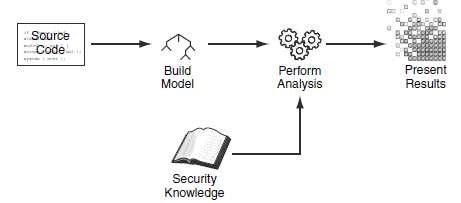
\includegraphics[scale=0.90]{img/static-code-analysis-internals}
		\caption{The process of static analysis, adopted from~\cite{secure-programming-sca}}
		\label{fig:static-code-analysis-internals}
\end{figure}


\subsection{Build a~Model}
In order to analyze the~program, the~analysis tool must first understand it. Therefore, the~initial task is to \textit{create a~structured model} that represents the~source code. This model has a~lot in common with the~AST and symbol tables that were discussed in Chapter~\ref{chap:compilers}. In fact, model building phase of static code analyzers closely mimics the~front end part of the~compilation process, executing lexical analysis, parsing and semantic analysis.

\subsection{Perform the~Analysis}
After obtaining the~model, the~next step is to perform the~actual analysis. Many different algorithms can be applied in this step and it is common that they are combined into one solution. The approaches are often derived from techniques used by the~compilers, specifically:

\subsubsection{\textbf{Control Flow}}
In order to explore different execution paths that can take place when the~program is executed, the~static code analysis tool can construct a~\textit{control flow graph} on the~top of the~AST. The nodes of the~graph represent basic blocks -- sequences of program instructions that will be all executed once block is entered. The edges between basic blocks represent different paths that the~program can take depending on matched conditions. Any back edges in the~graph signal potential loops in the~program execution.

\subsubsection{\textbf{Tracking Data Flow}}
Data flow analysis is used to examine how data passes through the~program. Compilers utilize data flow analysis when doing code optimizations in order to remove unreachable code and allocate registers. An example of how data flow analysis can be used by static analysis tools is to check that memory is always freed only once -- function \texttt{free(p)} was called at most once with the~address stored in pointer \texttt{p}.

\subsubsection{\textbf{Taint Analysis}}
According to~\cite{oswap-sca}, taint analysis attempts to identify variables containing possibly tainted user input using data flow analysis technique. If these variables are used as arguments to vulnerable functions without being sanitized first, the~tool reports their usage as vulnerable. The taint propagation analysis is particularly relevant for security analysis, a~prime example being the~detection of a~potential SQL injection.

\subsection{Rules}
As stated in~\cite{sca-for-security}: \textit{"...if a~rule hasn’t been written yet to find a~particular problem, the~tool will never find that problem."} This implies that the~rules that specify what the~static analysis tool should report are just as important (or even more important) as the~heuristics and algorithms implemented by the~tool. Best tools for static code analysis externalize the~rule set in order to easily add, remove or alter the~rules, without modifying the~tool itself.

\subsection{Report the~Results}
An often overlooked part of the~static analysis is the~result reporting. The~\cite{coverity-sca} asserts, that if a~programmer cannot understand the~output of the~static analysis, the~results are effectively useless as misunderstood explanation ends up with error being ignored or, worse, interpreted as a~false positive.

As discussed in~\cite{security-programming-sca}, good static analysis tool should provide means of \textit{grouping and sorting} the~results, \textit{suppressing the~unwanted results} (either directly in the~code with pragmas or code annotations or alternatively in a~configuration file) and mainly \textit{explaining the~results}. Every issue that is detected by the~tool should provide a~short title followed by a~detailed description of the~problem, severity of the~issue, recommendations on how the~problem can be fixed and possible further references to the~topic. The tool can additionally provide a~confidence level estimating the~likelihood that the~finding is really correct.

\section{What Problems Can Be Solved by SCA}
There are different types of problems the~static analysis tool can tackle. This section enumerates some of the~categories applicable to static code analysis, as listed in~\cite{secure-programming-sca}.

\subsubsection{\textbf{Type Checking}}
The integral part of every compiler for statically typed language. Rules are typically implied by the~language itself.

\subsubsection{\textbf{Style Checking}}
The style checker defines rules for spacing, naming, commenting and general program structure that affect mostly the~readability and the~maintainability of the~program. 

\subsubsection{\textbf{Program Understanding}}
These tools aim to provide a~high-level program understanding beneficial mainly for larger codebases. They are most effective when integrated into the~IDEs where they can support "go to declaration" or "find all references" features or even automatic program refactorings such as renaming or extracting a~variable.

\subsubsection{\textbf{Bug Finding}}
The  purpose of these type of static analyzers is to point out common mistakes in the~code. They report warnings in parts of program that are compliant with the~language specification but might not express the~programmer's intent, such as ignoring the~return value of a~function call.

Special type of bug finding checker is \textit{security review}, where specific vulnerabilities found in the~source code are reported. Security review searches for possible exploitations like buffer overflow or tainted inputs.
  
\section{Advantages}
One of the~key factors that advocate the~use of tools for static analysis, is how early in the~development process they can be applied. As opposed to dynamic testing, static code analysis can be performed on unfinished or even uncompilable code. The longer the~defect stays in the~system, the~more damage it can cause and the~higher are the~costs of fixing it. As stated in~\cite[p. 29]{code-complete}, the~costs of fixing a~defect introduced during construction of a~program are 10-times higher if detected during system testing and 10 to 25-times higher in production, than it would be to fix it while still in development. Therefore, it is desirable to detect bugs as early as possible, which is where static code analysis can be leveraged.

Static inspections detect symptoms together with causes whereas testing only points out the~symptoms with further effort required to find the~source of the~problem before it can be fixed~\cite[p. 472]{code-complete}.

Manual code inspections can be very time-consuming and require high level of expertise from the~reviewer. Static code analysis help to make the~code review process more efficient by checking for well-known flaws which do not have to be considered during code review.

Another advantage of automated code analysis is repeatability and scalability. Code analysis tool can be part of Continuous Integration\footnote{Process in which developers contribute regularly (multiple times a~day) into a~shared repository where the~code is continuously being verified by an~automated build and suite of automated tests.} (CI) process and can be also integrated to programming IDEs\footnote{Integrated Development Environment}. 

As such, they are a~great for programmers who get instant feedback and learn more about mistakes they made. The tools enforce higher code quality and guidelines compliance. As a~result, the~code should be more consistent, maintainable and easier to debug.
  
\section{Disadvantages}
The Rice's theorem~\cite{direct-proofs-of-rices-theorem} says, that any non-trivial question about program's semantics is undecidable. As a~consequence, there will never be a~static analysis tool able to answer all the~questions perfectly. The tools can produce \textit{false positives} (a problem which does not actually exist is reported) and \textit{false negatives} (the program contains a~problem, but it was not reported by the~tool).

Prevailing complaints against static analysis tools concern false positives. A long list of false positives means real bugs can be overlooked and programmers can eventually lose trust in the~tool.

Worse, from the~security perspective, are false negatives. Not only the~bug was not found and might cause future problems, but they also provide a~false sense of security to the~programmers. 

As presented earlier in this chapter, a~vast majority of code inspection tools must build a~model of the~source program in order to be able to analyze it. This requires duplication of compiler's logic, which itself is fairly complicated, and there is no guarantee that the~tool interprets the~source exactly the~same as the~compiler does. Moreover, for the~authors of the~tool, it means the~parsing logic has to be always up to date with the~language version in use. 

\section{Static Code Analysis Tools Available on the .NET Platform}
Even if imperfect, static analysis tools are still valuable asset in software development process. This section presents tools for static code analysis that are commonly used on the~.NET platform.

\subsection{FxCop}
FxCop is a~free tool by Microsoft for analyzing managed code assemblies (targeting .NET Framework) for conformance to .NET Framework Design Guidelines\footnote{\url{https://msdn.microsoft.com/en-us/library/ms229042(v=vs.110).aspx}} in areas such as design, localization, performance, security, naming or portability. 

It includes more than 200 predefined checks and a~possibility to add custom rules using FxCop SDK\footnote{Software Development Kit}. It is available in two forms: fully featured application with graphical user interface and a~command line tool that is easily integrated to automated build process. 

\subsection{StyleCop}
Another tool by Microsoft is an~open source project StyleCop\footnote{\url{https://github.com/StyleCop/StyleCop}} for analyzing C\# code for conformance to style and consistency with .NET Framework Design Guidelines. Unlike FxCop, StyleCop analysis is performed on the~source code, which enables it to look for a~different set of style violations. The rules are divided into categories such as documentation, naming, ordering, spacing and readability. 

Some of the~rules are: placing the~opening curly brace on a~new line, spaces around binary operators, method names starting with an~upper-case. The tool is configurable and development team can specify its own style to be checked, for example, to enforce spaces over tabs. It is available either a~Visual Studio extension or a~NuGet package that can be installed to the~project.

\subsection{CodeRush Classic}
CodeRush Classic\footnote{\url{https://www.devexpress.com/Products/CodeRush}} is a~solution-wide static code analysis tool for Visual Studio by vendor DevExpress. It enhances the~IDE with more advanced features like assembly decompilation, automated code generation, advanced code selection, code formatting and cleanup. The tool focuses on developer's productivity by not only finding bugs but also providing an~automated way of fixing them.

It provides an~API enabling developers to extend the~basic functionality with 3rd party plugins such as spell checker or copy project. The CodeRush Classic provides static analysis not only for .NET languages, but also for JavaScript, HTML and XML.

\subsection{Resharper}
Very similar to CodeRush, ReSharper is a~Visual Studio extension for .NET developers by Jet Brains\footnote{\url{https://www.jetbrains.com/resharper}}. It analyzes code quality of C\#, Visual Basic, ASP.NET, JavaScrtipt, TypeScript, CSS, HTML and XML. For each of these languages it is possible to define code style and formatting to make the~tool compatible with the~coding standards followed by a~development team. 

ReSharper provides hundreds of quick-fixes that solve discovered problems and has support for automated solution-wide refactorings. On the~top of static analysis there are additional plugins for performance (dotTrace) and memory (dotMemory) profiling, test runner and code coverage tool (dotCover) or .NET decompiler and assembly browser (dotPeek).


\subsection{Analyzers Written with Roslyn}
The tools described above have one aspect in common -- they all need to parse the~code before they can analyze it. The cost of maintaining a~custom C\# parser and keep it up to date with every new language version is fairly difficult, inefficient, and of course, costly. 

With the~release of new .NET Compiler Platform (Roslyn), which is discussed in detail in the~following chapter, the~need for parsing C\# and Visual Basic sources is eliminated and tools that build upon this platform can concentrate solely on analysis itself.

Some vendors, like Jet Brains, who invested years of development into the~creation of the~tools, claim ~\cite{resharper-and-roslyn-qa}, it does not pay off to rewrite the~whole program so that it uses new Microsoft compiler. Not only would it take an~enormous effort to rewrite all the~functionality to use new framework, but they would risk destabilizing the~product and losing years of optimizations and testing. Moreover, ReSharper is multilingual tool whereas .NET Compiler platform "only" provides C\# and Visual Basic parsers.

Other companies, such as DevExpress with CodeRush\footnote{CodeRush Classic referrs to the~version before Roslyn} or Microsoft with StyleCop Analyzers, decided to use this new approach. The effects on Visual Studio performance were immediate, since solution does not have to be parsed by the~tool, nor duplicate syntax trees stored. As a~result, the~load times and memory consumption were significantly lowered.

The Roslyn APIs also gave rise to more open source projects dealing with static code analysis, such as CodeCracker\footnote{\url{https://code-cracker.github.io}}. As challenging as it was in the~past, static code analysis is now rather easy, thanks to powerful analysis APIs. Following chapter takes a~look at the~.NET Compiler Platform and how it can be used to perform the~static code analysis.

% =================================================================
% ============================= CHAPTER 4 =========================
% =================================================================
\chapter{The .NET Compiler Platform}
In~the~.NET world, the~compiler used~to~be a~black box that given the~file paths to~the~source text, produced an~executable. This perception was changed in~2015 when Microsoft introduced the~.NET Compiler Platform (commonly referred to as "Project Roslyn").  

%\begin{figure}[h!]
%		\centering
%			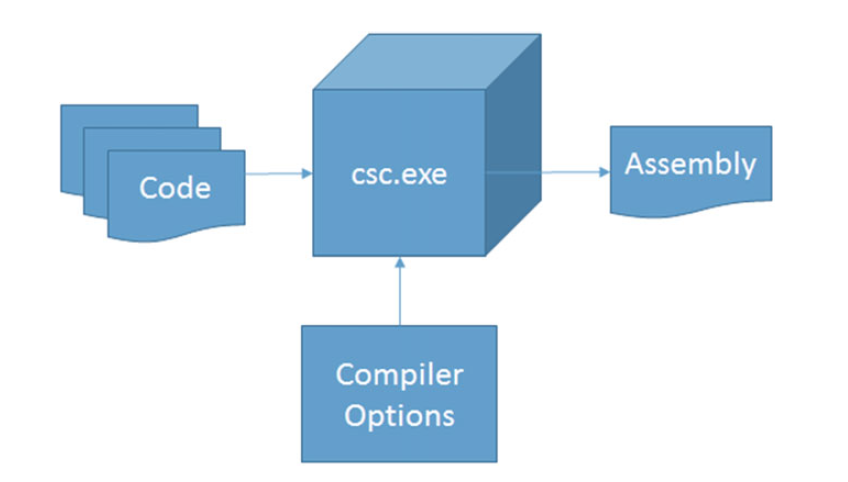
\includegraphics[scale=0.35]{img/compiler-as-a-black-box}
%		\caption{Compiler as a~black box~\cite{dot-net-development-using-the-compiler-api}}
%		\label{fig:compiler-as-a-black-box}
%\end{figure}

Not only have been compilers for both Visual Basic and C\# rewritten into the~entirely managed code\footnote{The term managed code refers to program source code written in one of high-level programming languages available for use with Microsoft .NET Framework, and require a~Common Language Runtime virtual machine in order to be executed.}, they also expose the~internals of the~compiler pipeline via a~public .NET API~\footnote{Application Programming Interface}. This makes them a~platform (also known as \textit{compiler-as-as-service}) with rich code analysis APIs that can be leveraged by developers to perform analysis, code generation or dynamic compilation in their own programs~\cite{roslyn-succinctly}. Those can be then easily integrated into Visual Studio all without the~hard work of duplicating compilers' parsing logic.

This chapter will take a~look at how the~Roslyn API layers are structured, how the~original source code is represented by the~compiler and how developers can build tools upon the~compiler's API. Note, that although Roslyn provides equivalent APIs for both VisualBasic and C\#, this thesis only focuses on the~latter since it is relevant for the~practical part of the~thesis.  
  
\section{The Compiler Pipeline}
Roslyn compilers expose an~API layer that mirrors the~traditional compiler pipeline (see Figure~\ref{fig:roslyn-compiler-pipeline}). Instead of a~single process of generating the~target program, each compilation step is treated as a~separate component~\cite{roslyn-overview}:

\begin{itemize}
  \item \textbf{Parse phase} consists of \textit{lexical analysis} (\textit{scanner}) and \textit{syntactic analysis} (\textit{parser}). First, the~lexical analyzer processes the~stream of characters from the~source program and groups them into meaningful sequences called \textit{lexemes}. Those are subsequently processed by the~\textit{syntax analyzer} that creates a~tree-like structure of tokens based on the~language grammar~\cite{dragon-book}.

  \item \textbf{Symbols and metadata phase} where named symbols are generated based on the~declarations from the~source and imported metadata.

  \item \textbf{Bind phase} in which the~identifiers from the~source code are matched to their respective symbols.

  \item \textbf{Emit phase} where all the~gathered information is used to emmit an~assembly.
\end{itemize}

\begin{figure}[h!]
		\centering
			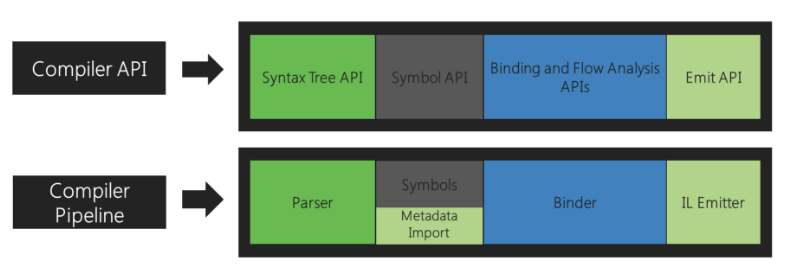
\includegraphics[scale=0.5]{img/roslyn-compiler-pipeline}
		\caption{Compiler pipeline~\cite{roslyn-overview}}
		\label{fig:roslyn-compiler-pipeline}
\end{figure}

In each phase, the~.NET Compiler Platform creates an~object model containing gathered information and exposes it through the~API in form of .NET objects. These objects are also used internally by Visual Studio~\footnote{The new generation of Visual Stuio leveraging from the~Roslyn compiler are called vNext and first one was VS 2015.} to support basic IDE functionality. For instance \textbf{syntax tree}, that is the~result of the~parse phase, is used to support formatting and colorizing the~code in the~editor. The result of the~second phase -- \textbf{hierarchical symbol table}, is the~basis for \textit{Object browser} and \textit{Navigate~to} functionality. Binding phase is represented as an~\textbf{object model that exposes the~result of the~semantic analysis} and is utilized in \textit{Find all~references} or \textit{Go~to~definition}. Finally, the~Emit phase produces the~Intermediate Language (IL) byte codes and is also used for \textit{Edit and~Continue} feature~\cite{roslyn-overview}.

\section{The .NET Compiler Platform's Architecture}
The Roslyn's architecture consists of two main layers - Compiler and Workspaces APIs, and one secondary layer - Features API, as seen on Figure~\ref{fig:roslyn-compiler-architecture}.

\begin{figure}[h!]
		\centering
			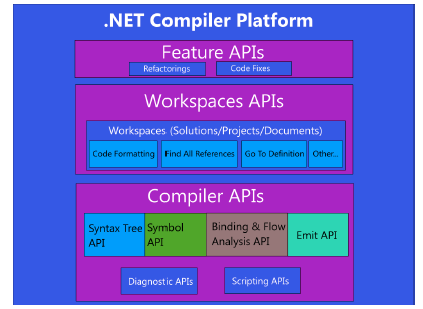
\includegraphics[scale=0.6]{img/roslyn-compiler-architecture}
		\caption{.NET Compiler Platform Architecture~\cite{roslyn-succincly}}
		\label{fig:roslyn-compiler-architecture}
\end{figure}

One of the~key concepts of .NET Compiler Platform is immutability. The compiler exposes hundreds of types that represent all information about source code from \texttt{Project} and \texttt{Document} to \texttt{SyntaxTrees} with almost all of those types being immutable. This means, that once created, the~object cannot change. In order to alter it in any way, new instance must be created, either manually, or from an~existing instance by applying one of many \texttt{With()} methods that the~API provides.

The immutability enables the~compiler to perform parallel work without need to create duplicate objects or apply any locks on them. This concept is useful for the~command line compiler but it is considered extremely important for IDEs where it enables for one document to be handled by multiple analyzers in parallel.

\subsection{The Compiler APIs}
As discussed in the~previous section, the~Compiler APIs offer an~object model representing the~results of syntactic and semantic analysis produced by the~respective phases of the~compiler pipeline. Moreover, it also includes an~immutable snapshot of a~single compiler invocation, along with assembly references, compiler options, and source files. This layer is agnostic of any Visual Studio components, and as such can be used in stand-alone applications as well. There are two separate, though very similar, APIs for Visual Basic and C\#, each providing functionality tailored for specific language nuances.

\subsubsection{\textbf{Diagnostic APIs}}
Apart from parsing code and producing an~assembly, the~compiler is also capable of raising diagnostics, covering everything from syntax to semantics, and report them as errors, warnings or information messages~\cite{roslyn-succinctly}. This is achieved through the~compilers' Diagnostics APIs that allow developers to effectively plug-in to compiler pipeline, analyze the~source code using the~exposed object models, and surface custom diagnostics along with those defined by the~compiler itself. These APIs are integrated to both MSBuild~\footnote{The Microsoft Build Engine \url{https://github.com/Microsoft/msbuild}} and Visual Studio (2015 and newer), providing seamless developer experience. Since the practical part of~this thesis, and~both Chapter~\ref{chap:custom-roslyn-analyzers} and~\ref{chap:performance}, rely on~Diagnostic APIs to~provide custom diagnostics, they are discussed in~more detail in~Section~\ref{sec:analyzers-and-code-fixes}.

\subsubsection{\textbf{Scripting APIs}}
As a~part of the~compiler layer, Microsoft team has introduced new Scripting APIs that can be used for executing code snippets. These APIs were not shipped with .NET Compiler Platform 1.0 and are part of v2.0.0 RC3\footnote{Release candidate 3, as per \url{https://github.com/dotnet/roslyn/wiki/Scripting-API-Samples} [26-02-2017].}.

\subsection{Workspaces APIs}
Workspace represents a~collection of solutions, projects, and documents. It provides a~single object model containing information about the~projects in a~solution and their respective documents; exposes all configuration options, assembly and inter-project dependencies, and provides access to syntax trees and semantic models. It is a~starting point for performing code analysis and refactorings over entire solutions.

Although it is possible to use the~\texttt{Workspace} outside of any host environment, the~most common use case is an~IDE providing an~instance of \texttt{Workspace} that corresponds to the~open solution. Since the~instances of \texttt{Solution} are immutable, the~host environment must react to every event (such as user key stroke) with an~update of the~\texttt{CurrentSolution} property of the~\texttt{Workspace}.

\subsection{Feature APIs}
This layer relies on both compiler and workspaces layers and is designed to provide API for offering code fixes and refactorings. Features APIs were also utilized while working on the~practical part of this thesis.
  
\section{Syntax Tree}
As mentioned in the~previous sections, the~product of the~syntactic analysis is a~syntax tree. It enables developers to work with the~code in a~managed way instead of working against plain text. Syntax trees are used for both analysis and refactorings, where the~new code is generated either manually or as a~modified version of the~existing tree. While being immutable, syntax trees are thread-safe and analysis can be done in parallel.

It is important to point out, that in a~same way the~compiler constructs a~syntax tree from the~source text, it is also possible to round-trip back to the~text representation. Thus, the~source information is always preserved in full fidelity. This means that every piece of information from source must be stored somewhere within the~tree, including comments, whitespaces or end-of-line characters, which is a~major difference to the~general concept of compilers discussed in Chapter~\ref{chap:compilers}.

Figure~\ref{fig:roslyn-syntax-tree} shows a~syntax tree of an~invocation expression as obtained from Syntax Visualizer\footnote{\url{https://roslyn.codeplex.com/wikipage?title=Syntax\%20Visualizer}} extension available in Visual Studio. This tool is useful for understanding how Roslyn represents particular language constructs and is widely utilized whenever one needs to analyze the~code. Following sections explain what are the~main building blocks of such syntax tree, referring to Figure~\ref{fig:roslyn-syntax-tree}.

\begin{figure}[h!]
		\centering
			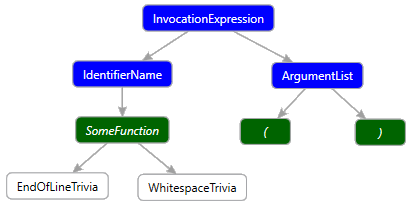
\includegraphics[scale=0.8]{img/roslyn-syntax-tree-2}
		\caption{Syntax tree of an~invocation expression}
		\label{fig:roslyn-syntax-tree}
\end{figure}

\subsubsection{\textbf{Syntax Nodes}}
Syntax nodes (blue color) are non-terminal nodes of a~syntax tree, meaning they always have at least one other node or token as a~child. Nodes represent syntactic constructs of a~language such as statements, clauses or declarations. Each type of node is represented by a~single class deriving from \texttt{SyntaxNode}. Apart from common properties \texttt{Parent}, \texttt{ChildNodes} and utility methods like \texttt{DescendantNodes}, \texttt{DescendantTokens}, or \texttt{DescendantTrivia}, each subclass exposes specific methods and properties. As shown in Figure~\ref{fig:roslyn-syntax-tree}, \texttt{InvocationExpression} has two properties, \texttt{IdentifierName} and \texttt{ArgumentList} both of which are \texttt{SyntaxNodes} themselves.
 
\subsubsection{\textbf{Syntax Tokens}}
As opposed to nodes, syntax token (green color) represent terminals of the~language grammar, such as keywords, punctuation, literals and identifiers. For the~sake of efficiency, \texttt{SyntaxToken} is implemented as a~value type (C\# structure) and there is only one for all kinds of tokens. To be able to tell them apart, tokens have \texttt{Kind} property. For example, \texttt{SomeFunction} is of kind \texttt{IdentifierName}, whereas "\texttt{(}" character is \texttt{OpenParenToken}.

\subsubsection{\textbf{Syntax Trivia}}
In order to enable refactoring features, syntax trees must also store information about whitespaces, comments and preprocessor directives that are insignificant for compilation process itself. This information is represented by another value type -- \texttt{SyntaxTrivia} (white color). Trivia are not really parts of the~tree itself, rather they are properties of tokens accessible by their \texttt{LeadingTrivia} and \texttt{TrailingTrivia} collections.

\section{Semantics of the~Program}
As explained in Chapter~\ref{chap:compilers}, even though syntax trees are enough to describe the~proper form of the~program (compliance to the~language grammar), they cannot enforce all language rules, for example, type checking. In order to tell whether a~method is called with the~right number of arguments, or operator is applied to operands of the~right type, it's inevitable to introduce semantics. 

Its one of the~core compiler's responsibilities to populate symbol tables with information about all elements and their properties from the~source program. Attributes such as identifier name, type, allocated storage, scope; or for method names the~number and types of arguments and their return values; are all stored in order to be utilized later when producing intermediate language.

\subsubsection{\textbf{Symbols}}
In .NET Compiler Platform, a~single entry of a~symbol table is represented by a~class deriving from \texttt{ISymbol}. The symbol represents every distinct element (namespace, type, field, property, event, method or parameter) either declared in the~source code or imported as metadata from a~referenced assembly. Each specific symbol has its own methods and properties often directly referring to other symbols. For example \texttt{IMethodSymbol} has a~\texttt{ReturnType} property specifying what is the~type symbol the~method returns.

\subsubsection{\textbf{Compilation}}
An important immutable type, that represents everything needed to compile a~C\# (or Visual Basic) program is a~\texttt{Compilation}. It contains all source files, compiler options and assembly references. Compilation provides convenient ways to access any discovered symbol. For instance, it is possible to access the~entire hierarchical symbol table rooted by global namespace, or look up type symbols by their common metadata names.

\subsubsection{\textbf{Semantic Model}}
When analyzing a~single source file of a~compilation, all its semantic information is available through a~\textit{semantic model}. The \texttt{SmeanticModel} object can answer many questions such as:
  \begin{itemize}
  \item What symbol is declared at the~specific location in the~source?
  \item What is the~result type of an~expression?
  \item What symbols are visible from this location?
  \item What diagnostics are reported in the~document?
  \end{itemize}
 
This makes semantic model very useful when performing static code analysis concerned with more than just syntax.
 
\section{Analyzers and Code Fixes}
\label{sec:analyzers-and-code-fixes}
Thanks to the Compiler APIs it is possible for Visual Studio to provide live static code analysis detecting any code issues as programmer types. Apart from general analyzers that are shipped with Visual Studio, it is possible to define custom, domain specific rules. The tricky task of running the analysis on background thread, showing squiggles in the IDE, populating the \textit{Error List}, and providing the \textit{light bulb} with code fix suggestions, is left to Visual Studio.

In order to understand the chapters describing the implementation part of the thesis, it is vital to know how the Diagnostic APIs work and how they are leveraged when writing a custom analyzer.

\subsection{Diagnostic Analyzer}
An analyzer is an instance of a type deriving from \texttt{Microsoft.CodeAnalysis.Diagnostics.DiagnosticAnalyzer} which must be annotated with \texttt{DiagnosticAnalyzer} attribute specifying the targeted programming language (C\# or Visual Basic)\cite{roslyn-succinctly}. In the text of this thesis, these instances are referred to as \textit{"end-analyzers"}, in order to distinguish them from abstract analyzers or helper classes containing analysis logic. The end-analyzer can contain one or more custom \textit{rules} for detecting domain specific errors or code issues. Each such rule is defined by \texttt{DiagnosticDescriptor}. Once the analyzer finds an issue, the diagnostic descriptor is used to create a \textit{diagnostic} which also includes data collected by the compiler, such as location.

\subsubsection{\textbf{Diagnostic Descriptor}}
For any Roslyn end-analyzer it is mandatory to override an immutable property \texttt{SupportedDiagnostics}. It returns an immutable array of diagnostic descriptors which consist of:

\smallskip
\begin{compactitem}
  \item[\texttt{\textbf{DiagnosticId}}] -- unique value identifying a single rule (e.g.~\textit{"BH103"}).
  \item[\texttt{\textbf{Title}}, \texttt{\textbf{MessageFormat}}, \texttt{\textbf{Description}}] -- localizable strings that will be displayed in Error List or diagnostic's tooltip on hover. The message format can be also passed arguments upon diagnostic creation, to give more details about the concrete issue detected.
  \item[\texttt{\textbf{Category}}] -- the category that the analyzer belongs to, such as code style, naming, design, etc. The list of categories defined for this thesis can be found in Section~\ref{sec:analyzer-categories}.
  \item[\texttt{\textbf{DefaultSeverity}}] -- one of \texttt{Error}, \texttt{Warning}, \texttt{Info}, \texttt{Hidden}, \texttt{None}. Note, that only \texttt{Error} severity prevents the project from compiling successfully.
  \item[\texttt{\textbf{IsEnabledByDefault}}] -- when this flag is set to \texttt{false}, the rule must be turned on manually in rule set editor.
  \item[\texttt{\textbf{HelpLinkUri}}] -- optional URI with online documentation.
\end{compactitem}

\subsubsection{\textbf{Performing the analysis}}
Besides providing the code that performs the actual analysis (commonly referred to as \textit{action}), it is necessary to register the action to tell the .NET Compiler Platform when to invoked it. To do so, the end-analyzer must override the \texttt{Initialize} method. This method represents the entry point of the analyzer and is invoked exactly once per \textit{session}\footnote{For batch compilations the session is a single run of the compiler. For hosted environments, where the analysis runs on the background thread, the session can last as long as the IDE is open. For more information see~\cite{analyzer-action-semantics}}. The method accepts one argument, of type \texttt{AnalysisContext}, exposing number of methods for registering actions. Depending on when the action should be invoked, a callback with analysis logic is passed to one of these methods~\cite{analyzer-action-semantics}:

\smallskip
\begin{compactitem}
  \item[\texttt{\textbf{RegisterSyntaxNodeAction}}] -- the action will be invoked on every syntax node encountered by the compiler if the kind of the node matches one of the kinds provided upon registration.
  
  \item[\texttt{\textbf{RegisterSymbolAction}}] -- the action will be invoked on complete semantic processing of a symbol that matches one of symbol kinds that the action was registered with.
  
  \item[\texttt{\textbf{RegisterSyntaxTreeAction}}] -- the action will be invoked as soon as whole document is parsed.
  
  \item[\texttt{\textbf{RegisterSemanticModelAction}}] -- the action will be invoked after the semantic analysis of the document is finished.
  
  \item[\texttt{\textbf{RegisterCompilationStartAction}}] -- the action will be invoked when the compilation starts (before any other actions). The context can be then used to register other actions within the compilation as well as the corresponding \texttt{RegisterCompilationEndAction}.
  
  \item[\texttt{\textbf{RegisterCodeBlockStartAction}}] -- action will be invoked before any of actions applicable to syntax nodes within the code block have been invoked. Optionally the analyzer might register the code block end action (\texttt{RegisterCodeBlockEndAction}).
  
  \item[\texttt{\textbf{RegisterCompilationAction}}], \texttt{\textbf{RegisterCodeBlockAction}} -- the~action will be invoked once per~compilations, or~code block, respectively.
\end{compactitem}

The compilation or code block start actions are usually registered for so called \textit{stateful analyzers}. These report diagnostics about specific code unit, as syntax node or a symbol (same as \textit{stateless analyzers}), but within the enclosing unit of code block or the compilation. They have to be designed carefully to perform effectively and not cause any memory leaks.

For both categories of analyzers it is vital to be written defensively and not to throw any exceptions. Otherwise, Visual Studio might disable it. An example of an analyzer detecting an access to the \texttt{Cookies} property of \texttt{HttpResponse} object can be seen in Figure~\ref{fig:analyzer-example}. It is actually a very simplified version of \texttt{HttpResponseCookiesAnalyzer} implemented for this thesis.

\begin{figure}[h!]
		\centering
			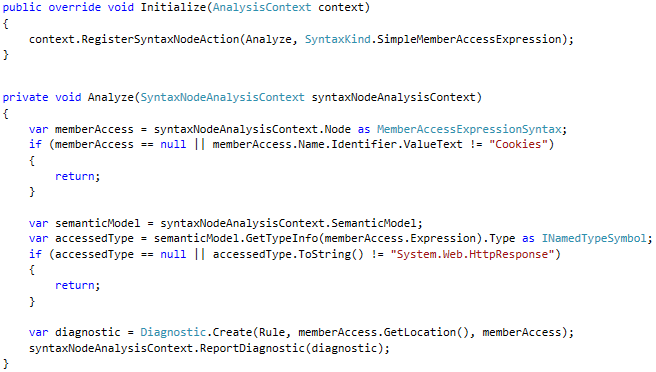
\includegraphics[scale=0.73]{img/analyzer-example}
		\caption{An example of a Roslyn analyzer syntax node analysis}
		\label{fig:analyzer-example}
\end{figure}

\subsection{Code Fix Provider}
A code fix is a quick action suggesting a possible solution to a diagnosed code issue found by the analyzer. It can be applied by invoking the quick actions (Ctrl+.) integrated into Visual Studio light bulb . Before applying, developer can view the live preview of the code fix action, as depicted in Figure~\ref{fig:codefix-example}.

\begin{figure}[h!]
		\centering
			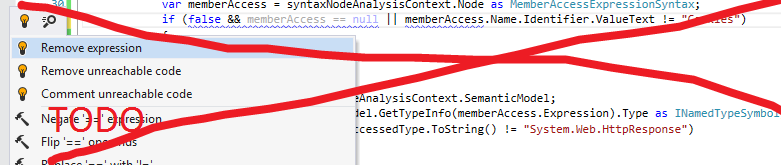
\includegraphics[scale=0.75]{img/codefix-example}
		\caption{A example of a code fix live preview}
		\label{fig:codefix-example}
\end{figure}

A custom code fix is defined by a class deriving from \texttt{Microsoft.CodeAnalysis.odeFixes.CodeFixProvider}. By overriding the \texttt{FixableDiagnosticIds} it claims which diagnostics it solves. The logic of fixing the diagnosed issue is placed in \texttt{RegisterCodeFixAsync} method, which ultimately generates whole new fixed document.

\section{Deployment}
There are two different approaches when it comes to deploying the analyzers and code fixes: NuGet package, or Visual Studio extension. 

With the IDE extension, every developer has to install it manually from Visual Studio Gallery\footnote{Visual Studio Gallery provides an access to various tools that extend the default Visual Studio functionality.}. Once installed, the analysis is performed on any open solution or project. Therefore, it is only appropriate for analysis concerned with common language or framework guidelines.

On the other hand, when tha analyzers are installed as a NuGet package. Only the project that has it installed will be analyzed. The reference to the NuGet is stored in shared repository, and everyone working with the project has the analyzers installed automatically. Moreover, only the NuGet installation influences the compilation process and, as such, can be run on build boxes as part of continuous integration process.

% =================================================================
% ============================= CHAPTER 5 =========================
% =================================================================


\chapter{Implementation of Custom Analyzers}
\label{chap:custom-roslyn-analyzers}
Kentico Software is an~IT company based in Brno, developing an~all-in-one solution for web content management, e-commerce, and online marketing, using the~ASP.NET\footnote{Open source framework for developing web applications by Microsoft.} architecture. The leading product is Kentico CMS (Content Management System). It has been on the~market since 2004 with the~11th version currently being developed. 

Over the~course of almost 13 years, the~solution grew to an~enormous extent. To give an~overview, the~current version of the~Kentico CMS solution contains 249   projects and a~total of 14,881 documents. A lot of knowledge was accumulated with many internal utilities developed and guidelines created. Many features, such as globalization, were developed in-house first, only to be added as an~integral part of the~.NET Framework a~few years later.

The size of the~company grew to more than 80 developers working on one product. It became significantly harder to share all the~knowledge about the~internal best practices and the~process of onboarding new employees was challenging. With the~increasing complexity of the~project, the~main focus of the~code reviews was shifted to the~general architecture and inspection of how the~new code influences the~other parts of the~system, in order not to break anything. The manual and often repetitive tasks of checking the~compliance with the~conventions and correct use of the~API during the~code review became very tiresome and dragged the~focus of the~reviewer away from the~higher perspective on the~code. This led to a~need for an~automated tool that would take care of the~repetitive checks that needed to be done by the~reviewer.

%company did not have the~motivation to invest too much into creating extremely complicated tool and at the~time (YYYY) it was very difficult to create something custom which would be robust and almost perfect at the~same time

%-  first attempts to rewrite BH to Roslyn 
%not so successful Bachelor thesis by another student (huge performance problems, implementation basically one to one with the~old console app, does not leverage of Roslyn type system, everything based on strings, therefore many missed diagnostic problems)

%why we are only concerned with this and do not check the~naming conventions or advanced refactoings - tools already exist for this (StyleCop and ReSharper) and were not implemented in new BH version - usings sorting and such is provided by other tools

% TODO tell how ReSharper or StyleCop are used in Kentico
\section{The Original BugHunter}
BugHunter is a~simple console application developed at Kentico that searches for violations of internal rules and best practices in the~the CMS solution. Given the~file path to the~solution folder, the~BugHunter performs the~checks and outputs the~results to a~file. Each issue found is reported with a~short message plus additional information on its location in the~code (source file and line number). It contains various checks not, only for C\#, but also a~few for JavaScript (like no skipped tests allowed), ASPX\footnote{TODO} (preferred usage of Kentico controls to default ones), or XML files.

Following sections explain the~main downsides of the~original BugHunter and how this thesis addresses them.

\subsection{Need for Semantic Analysis}
The biggest disadvantage of the~previous BugHunter was that the~tool performed the~checks purely by string comparison. It did not build any model of the~analyzed code and therefore possessed no knowledge of the~semantics. 

This caused an~enormous number of false negatives. A typical example would be the~tool trying to prevent the~access to the~\texttt{Cookies} property of the~\texttt{HttpRequest} object. The old BugHunter check looked something like this:

$$
if (line.Contains("Request.Cookies")) \\
\{
  \textnormal{// report an~error}
\}
$$

If the~programmer used the~most common approach\footnote{Accessing the~static property of the~class that is handling the~request.} of accessing the~\texttt{Cookies} collection on the~\texttt{Request} object, everything was fine and the~BugHunter correctly reported the~problem. However, it had no means of detecting other possible accesses to the~property. If the~\texttt{Request} object was passed to a~function as an~argument or stored in a~variable, the~accesses of the~cookies collection could not be detected by the~BugHunter. 

There were other use cases that could lead to false negatives when using just primitive string comparisons. For example, in C\# it is allowed to put an~arbitrary number of whitespace characters between the~object, the~dot token, and the~property being accessed. This could have been solved by using a~bit more complicated regular expression, but it would still cover only a~fraction of use cases. Things like using variable or even alias usings\footnote{\url{https://msdn.microsoft.com/en-us/library/aa664765(v=vs.71).aspx}} would stay undetected by the~tool. 

The only way to solve this was to introduce the~semantics into the~analysis which was a~relatively easy task for new Roslyn analyzers developed as part of this thesis.

\subsection{Ease of Use}
As mentioned in the~Chapter~\ref{chap:static-code-analysis}, the~key to success of a~static code analysis tool is the~ease of use. This means that running the~tool should not be complicated and interpreting the~results should be straightforward. If this is not the~case, programmers will not use the~tool or they will ignore the~results it produces. 

With the~original BugHunter, a~developer had to run the~separate application that took for about 30 seconds. Then, he or she had to analyze the~results before going back to the~IDE in order to look up the~reported issues and fix them. 

In a~discussion with the~developers at Kentico, they all admitted, that more often than not, they submitted the~changes to the~version control system without running the~BugHunter locally. 

The console application was run by the~build server itself as part of the~continuous integration. If the~BugHunter detected any issues, the~developer who caused them would be notified by an~email and would have to fix them as part of the~no-warning policy. This process prolonged the~time it took to finish the~implementation and generated a~demand for a~more developer-friendly solution. 

Since Roslyn analyzers are part of Visual Studio IDE, programmers get an~instant feedback and see the~warnings before submitting the~code without the~need to run an~external application.

\subsection{Suppressing the~Results}
Another downside of the~previous solution was the~way certain portions of the~code were excluded from the~analysis. Since the~BugHunter is a~console application and the~CMS solution is completely independent of it, the~configuration had to be placed in BugHunter's installation directory. This was deemed as not transparent, as it was not clear, why in one file certain code was okay, whereas, in the~other, it was reported as an~issue, without taking a~look into a~huge configuration file.

Moreover, the~only way to exclude a~certain piece of code from the~analysis was to put the~whole file, in which it appeared, into the~configuration of the~rule to be suppressed. This way of configuration lacked the~granularity and was opaque. 

On the~other hand, Roslyn provides numerous ways to turn off a~certain rule for a~project, a~file, or even a~line of code. More information on which approach was taken when deploying the~analyzers can be fount in the~Appendix~\ref{appendix:deployment}.

\section{Defining Analyzer Categories}
\label{sec:analyzer-categories}
The \texttt{Category} property of the~\texttt{Microsoft.CodeAnalysis.DiagnosticDescriptor} class provides a way for semantically distinguishing the~analyzers and giving additional information on what type of problem the~particular category is concerned with. The original BugHunter did not group the~checks into the~semantic categories but was structured rather by the~technology targeted by the~check (C\#, ASPX, JavaScript, web parts, etc.). 

Therefore, one of the~first tasks before the~implementation was to determine which checks are suitable candidates for refactoring into new Roslyn analyzers and subsequently group them into categories by the~type of the~task they performed. Basically, all the~checks that were not obsolete and were concerned with C\# internal guidelines were rewritten. Table~\ref{tab:analyzer-categories-compact-table} lists all implemented analyzers sorted into categories and following sections briefly elaborate on how the~categories were defined and what they represent. 

% ------------------ Summary Table ------------------
\begin{table}
\resizebox{1.005\textwidth}{!}{%
\begin{tabularx}{1.038\textwidth}{ll}
\toprule
\textbf{Category} & \textbf{Analyzer name} \\ \hline

\midrule
\textbf{AbstrOverImpl}
  & LuceneSearchDocumentAnalyzer \\

\textbf{CmsApiReplacements}
  & HttpSessionSessionIdAnalyzer \\
  & HttpSessionElementAccessAnalyzer \\
  & HttpRequestCookiesAnalyzer \\
  & HttpResponseCookiesAnalyzer \\
  & HttpRequestUserHostAddressAnalyzer \\
  & HttpRequestUrlAnalyzer \\
  & HttpRequestBrowserAnalyzer \\
  & HttpResponseRedirectAnalyzer \\
  & HttpRequestQueryStringAnalyzer \\
  & PageIsCallbackAnalyzer \\
  & PageIsPostBackAnalyzer \\
  & FormsAuthenticationSignOutAnalyzer \\
  & ClientScriptMethodsAnalyzer \\
  & SystemIOAnalyzer \\

\textbf{CmsApiGuidelines}
  & WhereLikeMethodAnalyzer \\
  & EventLogArgumentsAnalyzer \\
  & ValidationHelperGetAnalyzer \\
  & ConnectionHelperExecuteQueryAnalyzer \\
 
\textbf{CmsBaseClasses}
  & ModuleRegistrationAnalyzer \\
  & WebPartBaseAnalyzer \\
  & PageBaseAnalyzer \\
  & UserControlBaseAnalyzer \\

\textbf{StringAndCulture}
  & StringManipulationMethodsAnalyzer \\
  & StringEqualsMethodAnalyzer \\
  & StringCompareToMethodAnalyzer \\
  & StringStartAndEndsWithMethodsAnalyzer \\
  & StringIndexOfMethodsAnalyzer \\
  & StringCompareStaticMethodAnalyzer \\
\bottomrule
\end{tabularx}
}
\caption{Analyzers sorted into categories}
\label{tab:analyzer-categories-compact-table}
\end{table}
% ---------------------------------------------------

\subsection{Abstraction over Implementation}
Analyzers in this category check that there is no "hard reference" on third party libraries in the~code. Violation of this rule would require clients to use a~particular version of the~library which might collide with the~references on other components they are using, resulting in so-called "dependency hell"\footnote{\url{https://devnet.kentico.com/articles/referencing-multiple-versions-of-the-same-assembly-in-a-single-application}}. Therefore, in CMS solution the~hard references are replaced with a~thin layer of interfaces and adapters. The analyzers make sure, only the~interfaces are used throughout the~solution.

\subsection{CMS API Replacements}
In Kentico CMS solution there are many helpers that encapsulate the~traditional .NET API and might provide an~extended functionality. For example, determining the~current browser of the~user can be done by accessing the~\texttt{Browser} property of the~\texttt{HttpRequest} object. However, if this attempt fails there are still other ways to resolve it and the~CMS API typically has a~helper for such cases. The analyzers detect accesses to members that have an~equivalent in CMS API and suggest code fixes. 

\subsection{CMS API Guidelines}
These analyzers impose internal guidelines on the~CMS API usage. They forbid the~direct access to database from presentation layer (\texttt{ConnectionHelperExecutequeryAnalyzer}), point out usages of methods that may have more suitable or a~safer alternatives1 (\texttt{WhereLikeMethodAnalyzer} or \texttt{ValidationHelperGetAnalyzer}), or guide developers to use predefined constants where possible (\texttt{EventLogArgumentsAnalyzer}).

\subsection{CMS Base Classes}
Similar to CMS API Replacements category, the~analyzers search for classes that inherit from standard .NET classes with CMS alternatives and suggest the~correct CMS replacements.

\subsection{String and Culture}
This category of analyzers makes sure that string comparison\footnote{\texttt{Equals()}, \texttt{Compare()}, \texttt{IndexOf()} and their variants} and manipulation\footnote{\texttt{ToLower()}, \texttt{ToUpper()}} methods are always used with the~overload specifying \texttt{StringComparison} or \texttt{CultureInfo} parameter explicitly. This is vital for an~application like CMS that is used with culture specific data. For more information on what issues can be caused when not following this rule, like the~\textit{"Turkish-I problem"}, see \cite{best-practices-for-using-strings-in-dot-net}. 

\section{API Replacement Analyzer}
The CMS API Replacement category contains 15 analyzers which represents almost one half of total 31 analyzers that were created. Vast majority of these analyzers search for a~particular member being accessed or invoked on a~particular type. Any such usage found by the~analyzer shall be reported as CMS API contains a~replacement for it, with a~code fix suggested where applicable.

In order to prevent code duplication and ease the~process of adding new analyzers, the~analysis logic for the~analyzers in this category was extracted into two helper classes: \texttt{ApiReplacementForMemberAnalyzer} and \texttt{ApiReplacementForMethodAnalyzer}. These are instantiated and configured by the~concrete end-analyzer to perform the~analysis on their behalf.

\subsection{Configuration}
There are only a~few things the~API replacement analyzer need to know in order to perform the~actual analysis. This information is encapsulated in \texttt{ApiReplacementConfig} object. The object is passed as a~constructor argument upon creation of the~API replacement analyzer. It contains following properties:

\begin{itemize}
  \item \texttt{ForbiddenMembers} -- member names to look for (e.g. \texttt{"Cookies"}), 
  \item \texttt{ForbiddenTypes} -- names of fully qualified (super)types the~members belong to\footnote{The forbidden type is treated as the~highest type in the~inheritance hierarchy the~member could belong to.
} (e.g. \texttt{"System.Web.HttpRequest"}), 
  \item \texttt{Rule} -- an~instance of \texttt{DiagnosticDescriptor} that defines the~diagnostic raised upon detection of a~forbidden usage.
\end{itemize} 

The main reason behind \texttt{ForbiddenTypes} being an~array of strings rather than a~single string, is the~lack of inheritance hierarchy between \texttt{HttpRequest} and \texttt{HttpRequestBase} objects in the~.NET framework. They basically contain the~same members but do not derive from one another\footnote{More information on why this is so can be found in \url{https://msdn.microsoft.com/en-us/library/system.web.httprequestwrapper.aspx}} and therefore, the~analyzer must treat both types separately. 

On the~other hand, allowing for multiple forbidden members on one type under one diagnostic ID may also make sense, which is why \texttt{ForbiddenMembers} are also defined as an~array.

\subsection{Analyzer for Member Replacement}
The task for the~\texttt{ApiReplacementForMemberAnalyzer} is to subscribe to all possible member accesses and analyze them. If the~particular access is regarded as forbidden, given the~configuration supplied (\texttt{ApiReplacementConfig} object), the~analyzer raises a~diagnostic.

It is not enough for the~analyzer to subscribe only to \texttt{SimpleMemberAccessExpression} syntax kind. It also needs to analyze the~\texttt{ConditionalAccessExpression} (null conditional operator, '\texttt{?.}') which is a~new C\# 6.0 language feature\footnote{\url{https://msdn.microsoft.com/en-us/library/dn986595.aspx}}. 

Even though it would be possible to subscribe to both kinds of syntax nodes with one callback, the~underlying syntax of these two is so much different, it would make the~code cluttered and full of if-statements. Moreover, if Microsoft decides to add another possibility to access members in next language version, the~existing code would have to be modified.

Therefore, it was decided to encapsulate the~strategies for analyzing a~particular syntax node into separate classes. The API replacement for member analyzer instantiates the~strategy helpers, configures them, and tells them to run the~analysis methods as callbacks subscribed syntax node of a~particular kind. This makes the~code easily extendible.

\begin{figure}[h!]
		\centering
			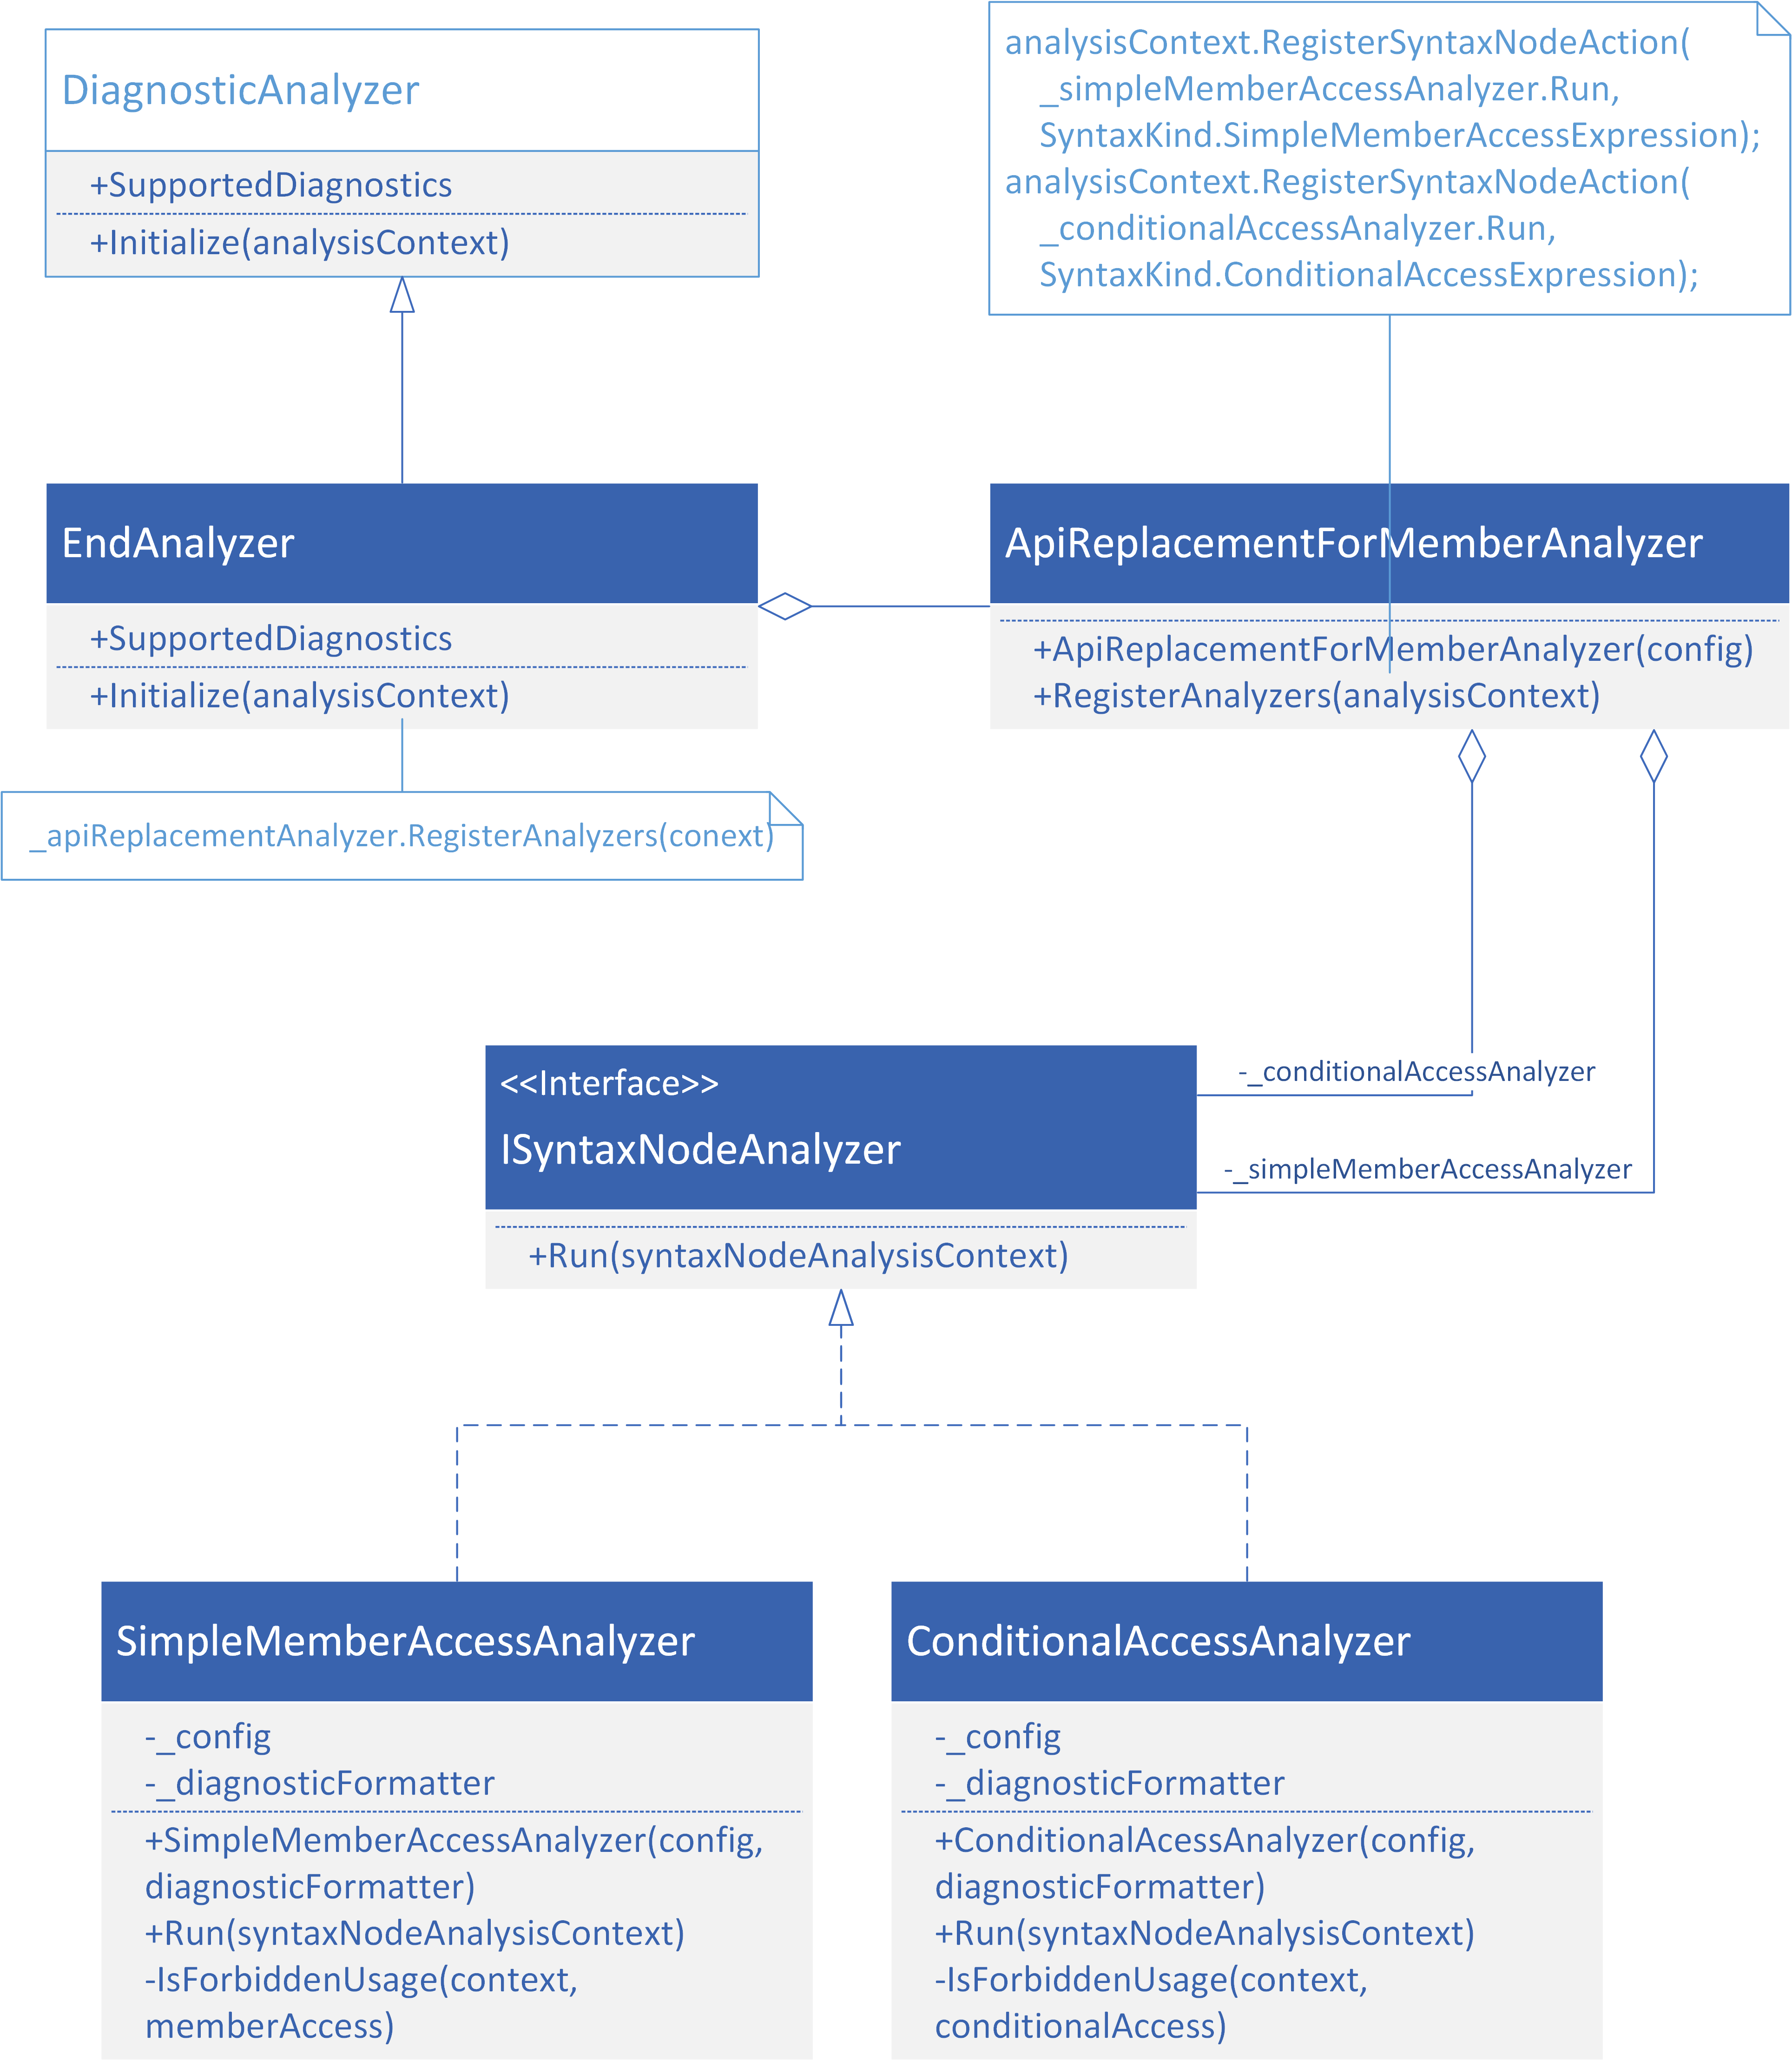
\includegraphics[scale=0.8]{img/uml/api-replacement-for-member}
		\caption{Class diagram for \texttt{ApiReplacementForMemberAnalyzer}}
		\label{fig:uml-api-replacement-for-member}
\end{figure}

The UML class diagram for \texttt{ApiReplacementForMemberAnalyzer} is depicted in Figure~\ref{fig:uml-api-replacement-for-member}. Note, that the~\texttt{DiagnosticAnalyzer} is an~abstract class defined in the~.NET Compiler Platform Diagnostics API and must be extended by the~custom end-analyzers.

\subsection{Analyzer for Method Replacement}
The class \texttt{ApiReplacementForMethodAnalyzer} is very similar to analyzer for members that was introduced in the~previous section. It also accepts a~configuration object defining the~invocations of which members on which types are forbidden. 
Instead of subscribing to member accesses it is interested in syntax nodes of kind \texttt{InvocationExpression}. It delegates the~analysis itself to a~strategy defined in \texttt{MethodInvocationAnalyzer}, described in the~following section.

\section{Method Invocation Analyzer}
This analyzer helper defines an~algorithm for analyzing invocation expression syntax nodes. The need for analyzing the~method invocations is not limited to the~API replacements. The same analysis needs to be performed when enforcing internal guidelines that are concerned with methods. It is important to locate the~specific methods invoked on specific types, before it is possible to analyze further whether or not they are used according to the~internal API conventions. 

\subsection{Template Method Pattern}
This analyzer is utilized by all end-analyzers that involve method invocation analysis. In order to be easily extendible for advanced checks, it is implemented as a~template method pattern\footnote{\url{http://www.oodesign.com/template-method-pattern.html}}. Every step of the~template method defines a~criteria that must be met in order for the~analysis to proceed. Steps that can be overridden have default implementation that continues with the~analysis. 

It is important to note that the~steps are ordered in a~way so that the~inexpensive checks are performed first, in order to cut off the~analysis of the~irrelevant nodes without significant performance costs. Figure~\ref{fig:uml-method-invocation-analyzer} shows the~class diagram of the~\texttt{MemberInvocationAnalyzer} depicting the~use of template method design pattern. Following section elaborate on respective steps of the~algorithm. Concrete use case depicting an instance of the analyzer can be seen in Figure~\ref{fig:uml-method-invocation-analyzer-object-diagram}.  

\begin{figure}[h!]
		\centering
			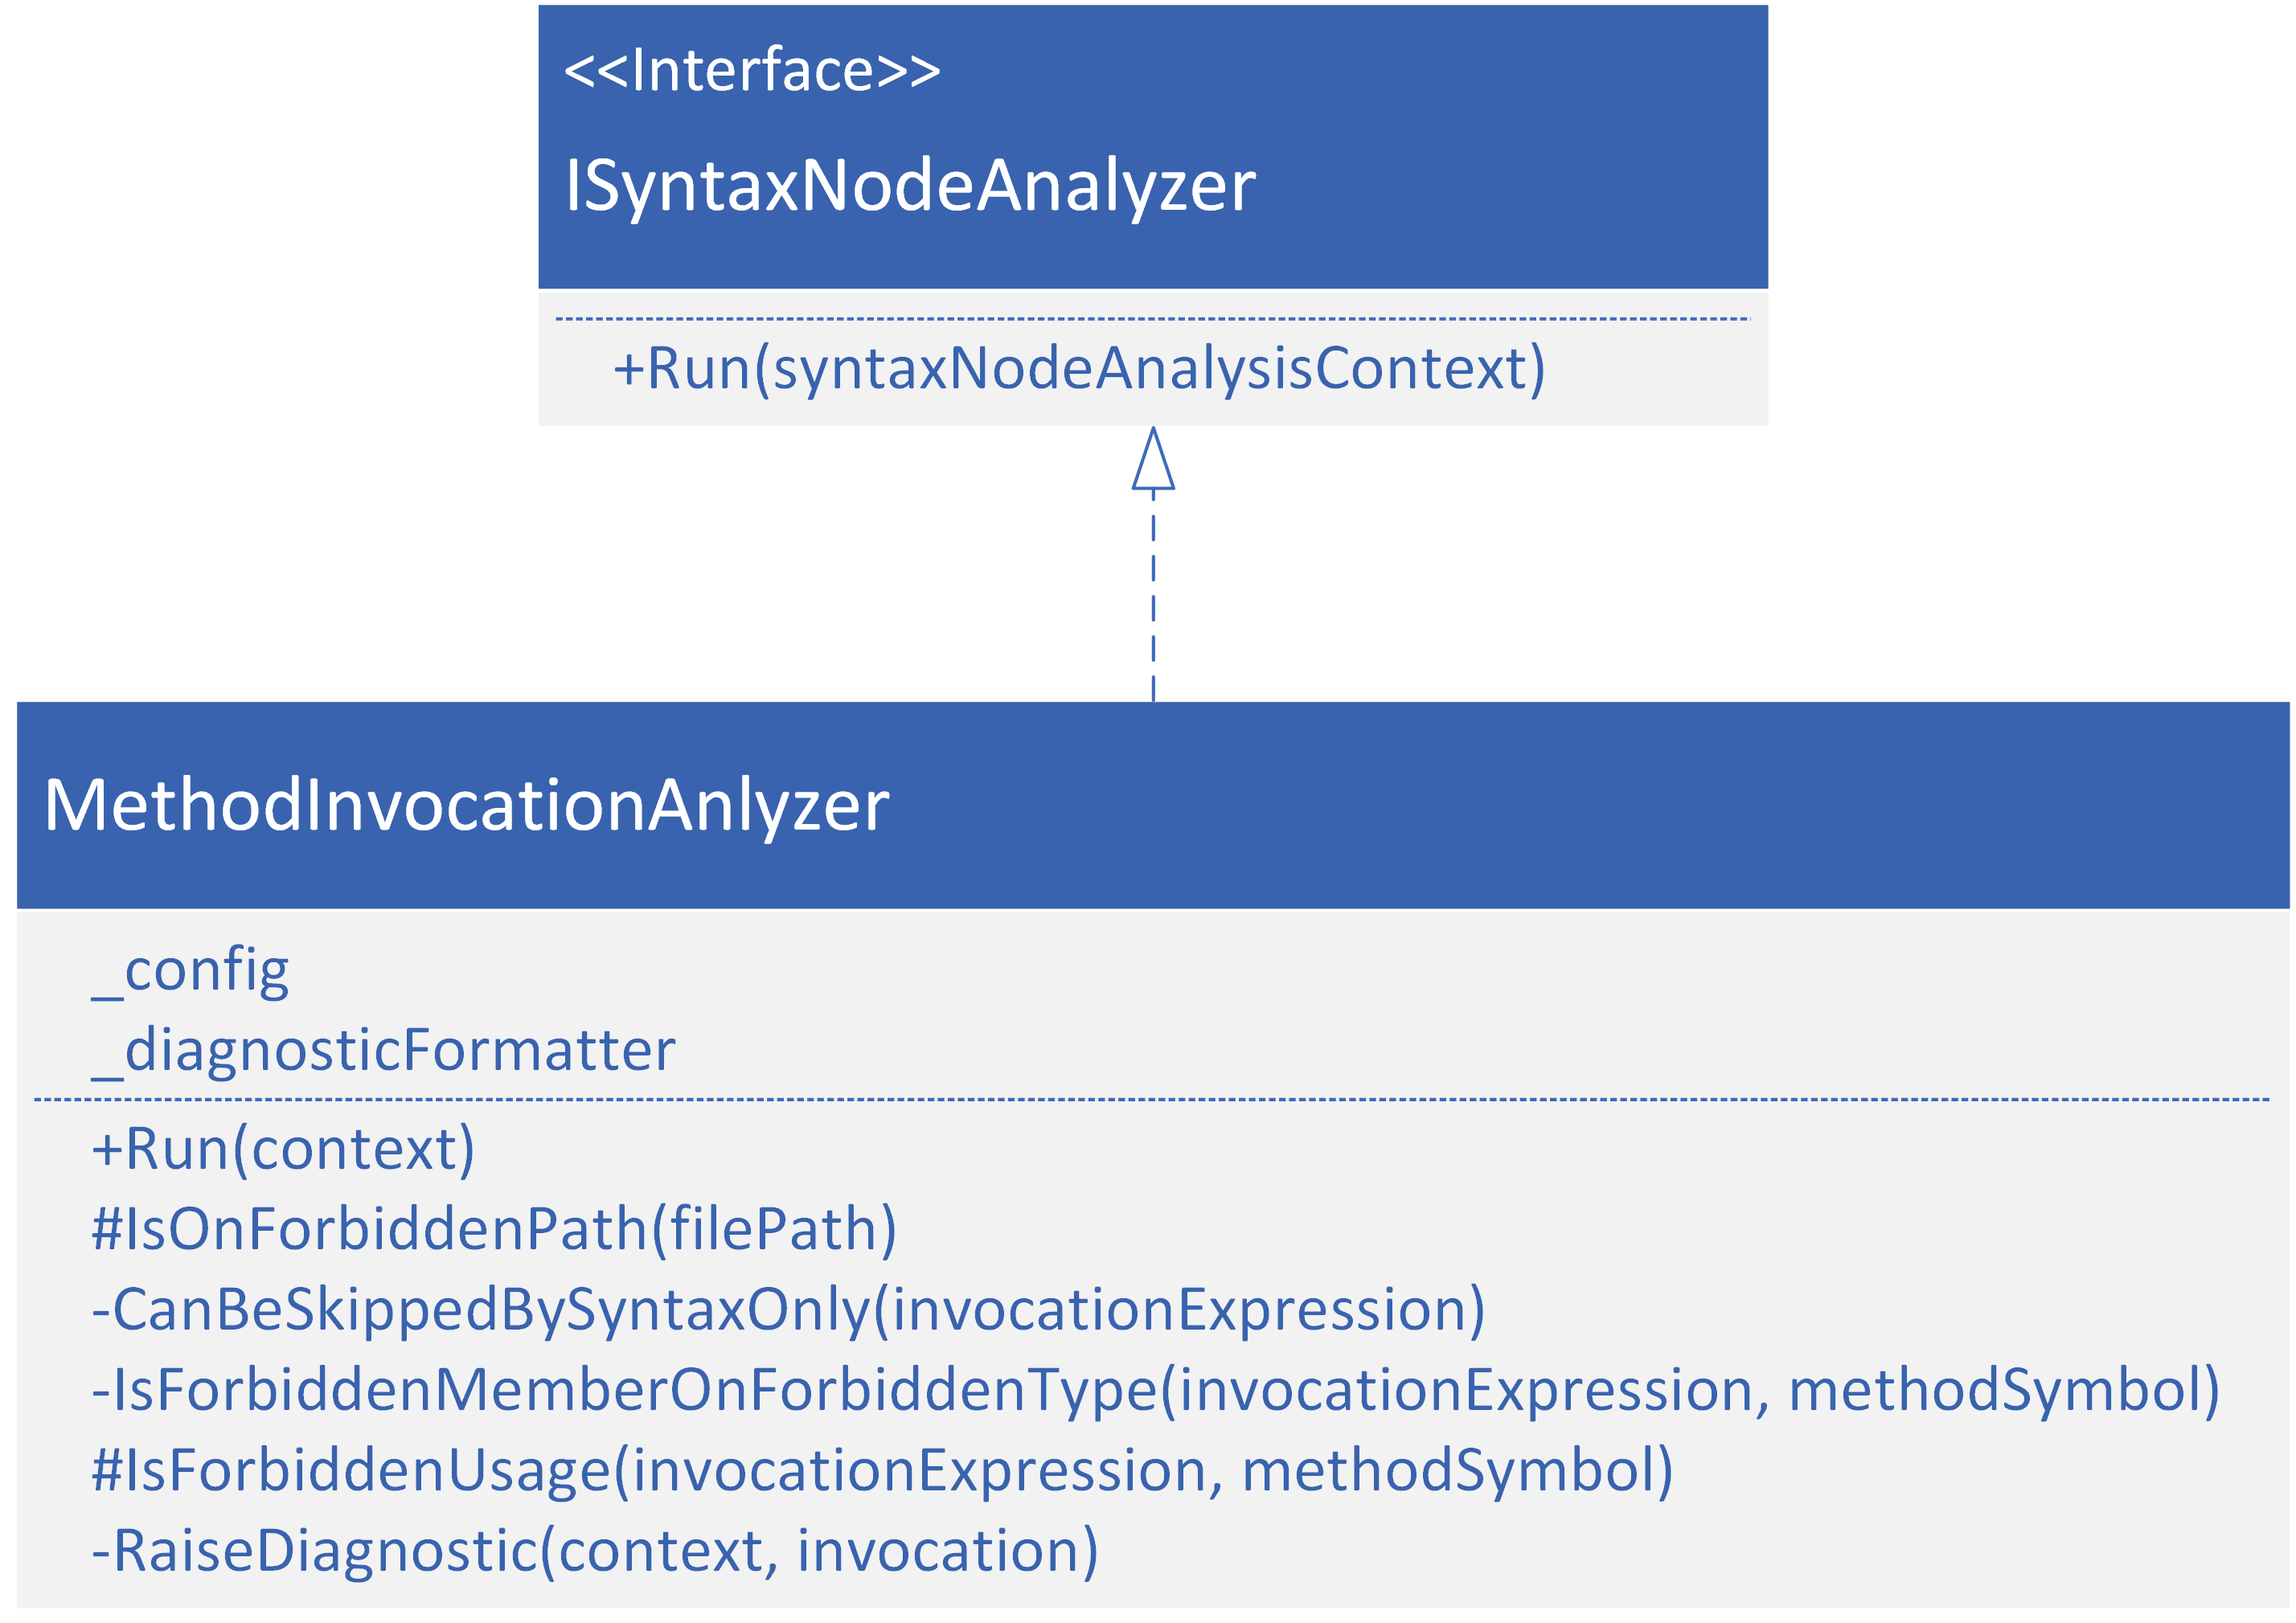
\includegraphics[scale=0.85]{img/uml/method-invocation-analyzer}
		\caption{Class diagram for \texttt{MethodInvocationAnalyzer} depicting the~template method design pattern}
		\label{fig:uml-method-invocation-analyzer}
\end{figure}

\subsubsection{\textbf{Check the~File Path}}
Sometimes, an analyzer needs to pre-filter files that are relevant for the~diagnostic. For example, when looking for an~access to the~database layer from the~presentation layer, the~analyzer is only concerned with the~invocation expressions in the~files of presentation layer. These can be identified by inspecting the~\texttt{FilePath} property of the~\texttt{SyntaxTree} in which the~current invocation expression is located. If the~file path does not meet the~requirements, the~current invocation expression does not need to be analyzed further.

\subsubsection{\textbf{Method Name Syntax Analysis}}
This step exists purely for performance optimization reasons and cannot be overridden by subclasses. It tries to extract the~name of the~method invoked and compares it to the~forbidden members. If the~method name is not among the~forbidden members, the~algorithm stops and no expensive operations had to be done. Otherwise, the~algorithm advances to the~next step.

Since there are no constraints for what kind of syntax node the~\texttt{Expression} property of the~\texttt{InvocationExpressionSyntax} node could be, the~logic had to be implemented by hand. The heuristc inspects these three cases:
\begin{itemize}
  \item \textbf{Identifier name} -- the~simplest case where the~method being invoked is a~member of the~enclosing class.

  TODO example + graph
  
  \item \textbf{Simple member access expression} -- invocation on member that is being accessed on object, or class. Accesses can be possibly chained.
  
  TODO example + graph 
    
  \item \textbf{Conditional access expression} -- similar to the~previous case but the~access is conditional. The whole syntax tree is right-folded as opposed to the~simple member access left-folded syntax tree.
  
  TODO example + graph
  
\end{itemize} 
%TODO: it is easy to access semantic model first and analyze the~IMethodSymbol... however.. point out how many times this callback is invoked and how many times SemanticModel would have been queried... therefore very simple semantic for getting rid of cases that do not have to be analyzed further... tell about the~possible cases of InvocationExpression - nested SimpleMemberAccess.. first MemberBindingExpression, or IdentifierName... always show a~graph... if it could be skipped based on syntax - invoked method name is for sure none of the~forbidden member names, skip, otherwise, analyze further based on semantics

%!!!!do some benchmarking how this heuristic helped with the~performance!!!! show graph

\subsubsection{\textbf{Method Name and Receiver Type Semantic Analysis}}
Here, semantic model is queried for \texttt{IMethodSymbol} that matches the~analyzed \texttt{InvocationExpressionSyntax}. If the~method symbol is found, its property \texttt{Name} is checked against forbidden member names. If the~check passes, the~property \texttt{ReceiverType} is inspected and only if it is one of forbidden types or its subtype, the~algorithm proceeds. 

This method cannot be overridden as it is the~integral part of the~whole algorithm. It is also the~most expensive one, since the~checks in this method are performed on symbols obtained by querying the~semantic model. However, thanks to the~heuristics from the~previous step, the~majority of irrelevant cases was already filter out.

\subsubsection{\textbf{Context of the~Invocation Usage}}
If it is important to analyze the~specificities of the~invocation usage (mainly the~arguments supplied), the~subclasses can override \texttt{IsForbiddenUsage()} virtual method. The template method supplies it with two parameters: the~invocation expression and the~method symbol obtained in the~previous step.

\subsubsection{\textbf{Diagnostic Creation}}
If all the~steps above determined the~analyzed invocation is forbidden, the~last step of the~template method makes sure the~diagnostic is raised, using the~diagnostic descriptor provided upon creation. It is possible to configure the~diagnostic creation by providing optional instance of \texttt{IDiagnosticFormatter}. It is an~interface defined in \texttt{BugHunter} project that determines how the~diagnostic of certain syntax nodes shall be formatted (location and message text of the~diagnostic).

\subsection{Usage}
\label{sec:method-invocation-analyzer-usage}
Prime example how to use this template method is \texttt{EventLogArgumentsAnalyzer}, depicted in~Figure~\ref{fig:uml-method-invocation-analyzer-object-diagram}. It defines an~inner class that subclasses the~\texttt{MethodInvocationAnalyzer}, overriding its \texttt{IsForbiddenUsage()} method.

Then, this inner class is utilized by the~end-analyzer (\texttt{EventLogArgumentsAnalyzer}) to perform the~analysis. Upon instantiation the~end-analyzer provides it with~a~configuration object and a~custom diagnostic formatter. 
\begin{figure}[h!]
		\centering
			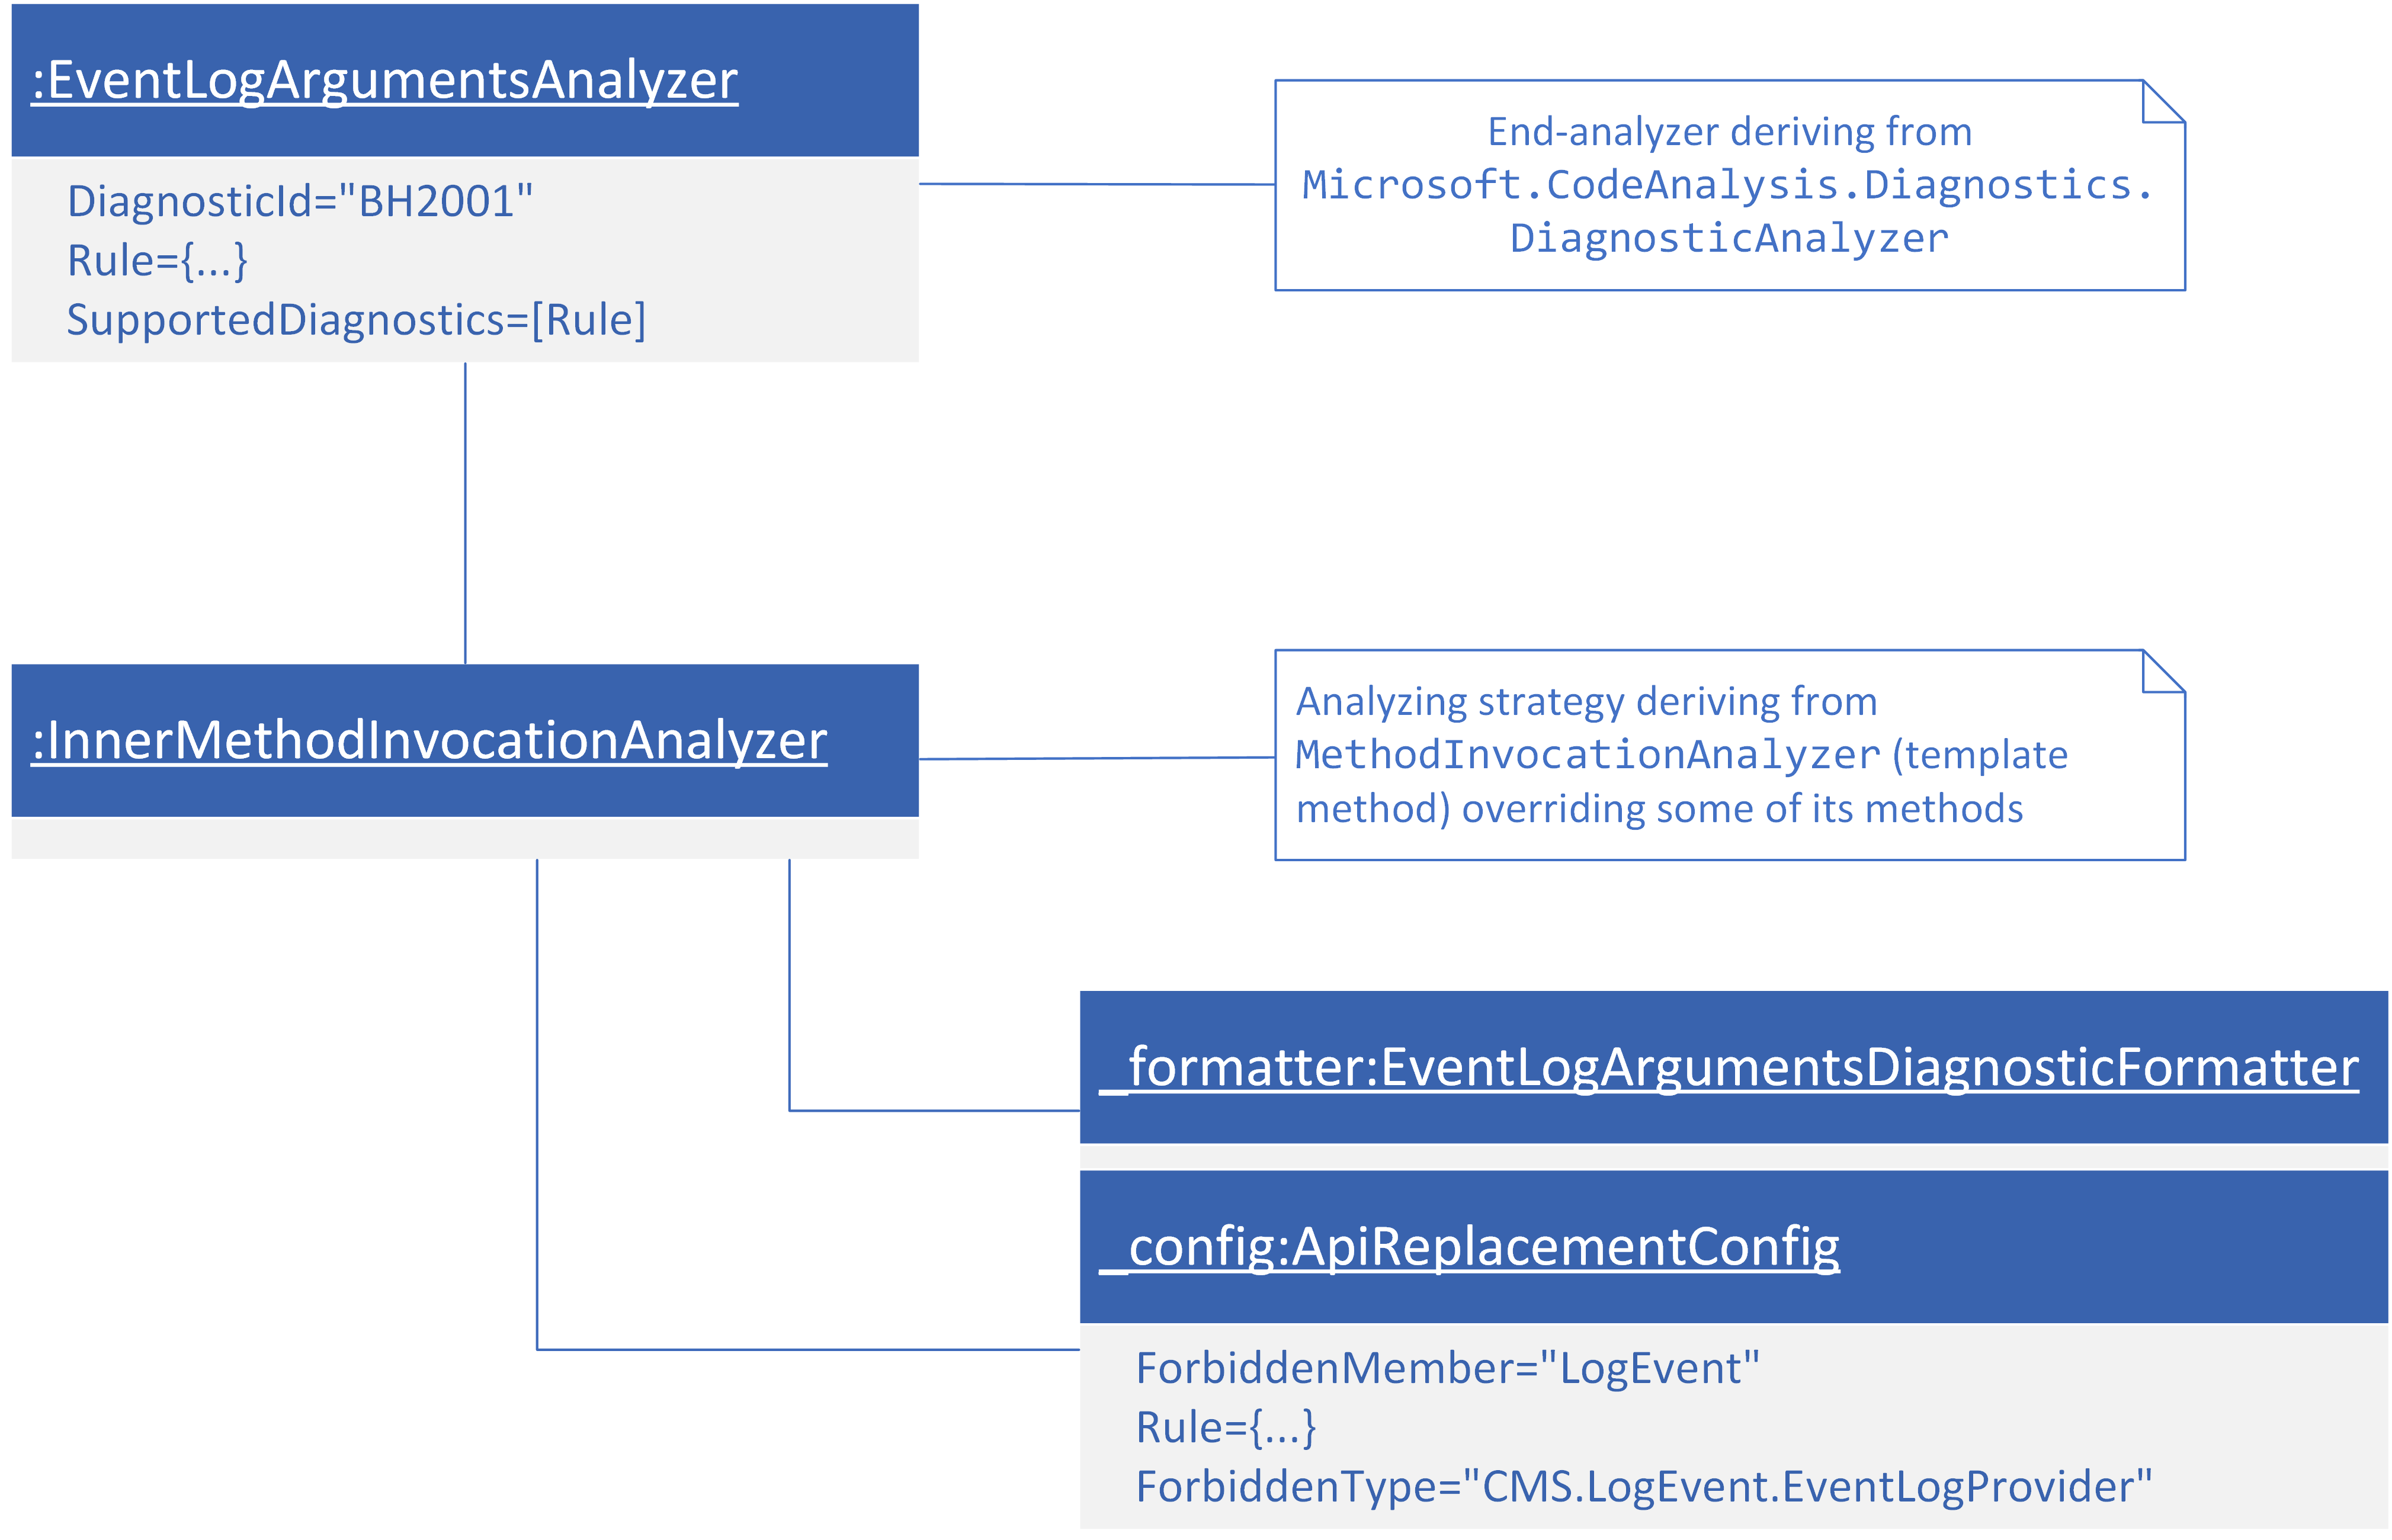
\includegraphics[scale=0.75]{img/uml/method-invocation-analyzer-object-diagram}
		\caption{Object diagram for \texttt{EventLogArgumentsAnalyzer} using inner class that derives from \texttt{MethodInvocationAnalyzer}}
		\label{fig:uml-method-invocation-analyzer-object-diagram}
\end{figure}

\subsection{Analyzers for String and Culture Checks}
The analyzers in this category search for methods like \texttt{Equals()}, \texttt{CompareTo()}, or \texttt{IndexOf()}. Considering that methods with same names can be found on many other types as well (\texttt{Object}, \texttt{Collection}), the~first syntax check for method name will often fail to filter out the~unrelated usages. Although all these analyzers could use the~\texttt{MethodInvocationAnalyzer} as a~strategy, it was decided to take a~different approach here. 

The fact that they only need to analyze the~invocations on the~\texttt{String} type, makes the~complex analysis of the~forbidden types in \texttt{MethodInvocationAnalyzer} ineffective. String is a~sealed class\footnote{Sealed classes cannot be subclassed.}, and so no complicated traversal of inheritance hierarchy is needed. In fact, in C\# strings are a~\textit{special type} and therefore, only a~simple check like this is sufficient:
$$
receiverType.SpecialType == SpecialType.System\_String
$$

\section{Code Fixes}
\label{sec:code-fixes}
All analyzers that were implemented provide one or more code fixes. There are only two exceptions:
\begin{itemize}
  \item \texttt{SystemIoAnalyzer}, since there is no one to one mapping between \texttt{CMS.IO} and \texttt{System.IO} APIs so it is not feasible to provide a~code fix in every situation,
  \item \texttt{ConnectionHelperExecuteQueryAnalyzer}, which a~detects database access from presentation layer that points out a~possible design flaw without an~automated solution.
\end{itemize} 

% TODO consider deleting this
The code fixes have one significant limitation -- providing a~fix to an~API replacement when the~forbidden access is conditional. This is due to the~nature of the~C\# grammar and the~way how null conditional operator is represented in the~syntax tree. If the access is chained, it would be very difficult to define the exact part of the syntax tree that should be replaced. In fact, there is even an issue\footnote{\url{https://github.com/dotnet/roslyn/issues/3110}} on GitHub of the Roslyn team explaining in detail why this is problematic. 

Therefore, it was decided not to provide the~code fix in such complicated cases. There were two ways for preventing code fix from being suggested. First one was to give the~diagnostic on conditional access different diagnostic id from the~easily-fixable member access. This was deemed as not particularly user friendly and other options were sought.

The approach taken was to provide an~additional information to the~diagnostic via the~\texttt{Properties} property\footnote{\url{http://www.coderesx.com/roslyn/html/93197CDD.htm}}. It is a~data structure were arbitrary key-value pairs can be stored when diagnostic is raised and can be later read in the~code fix class. The analyzer stores a~flag, telling the~diagnostic is raised for conditional member access. When the~code fix method is invoked, it can decide whether or not it is capable of providing a~fix for the~specific conditional member access.

\section{Tests}
Since it is infeasible to test the~functionality of all the~analyzers manually by running Visual Studio, it is crucial that all the~requirements are covered by an~automated set of tests. 

Every analyzer and its code fixes have an~extensive suite of tests covering the~functionality. The extension methods and helper classes are covered by separate unit tests as well. The pre-generated boilerplate from Visual Studio for testing analyzers was reused and rewritten using NUnit framework~\footnote{Testing framework for .NET languages \url{https://www.nunit.org}}. Since the~default template did not allow to set anything apart from the~sources, it had to be customized and some additional features were added.

A typical scenario for testing an~analyzer is to:
\begin{compactenum}
  \item Prepare the~source documents to be tested. Typically one C\# class stored in a~string.
  \item Create a~compilation out of the~source documents.
  \item Run the~analyzer under test on the~compilation.
  \item Compare the~output of the~analyzer with the~expected diagnostics.
\end{compactenum}

To test the~code fix, it is run on the~source containing a~diagnostic and the~document with applied code fix is compared to the~expected result.

\subsubsection{\textbf{Referencing Kentico Libraries in Tests}}
As can be seen, when testing analyzers and code fixes, the~compilation is always created from the~source documents. For this to work, all references to the~libraries used by the~source code, or relied upon by the~tested analyzer, need to be linked. This contains not only the~Microsoft core assemblies that are always added, but in case of the~BugHunter analyzers, also Kentico libraries. Therefore, the~default testing template had to be enhanced with the~ability to explicitly reference desired DLLs in the~created compilation.

\subsubsection{\textbf{Faking File Information of Documents in Compilation}}
The outcomes of some analyzers are dependant on the~file path of the~analyzed document. Therefore, to test them, it is necessary to be able to fake the~name of the~source document that will be part of the~analyzed compilation. To accommodate this requirement, the~the testing template was extended with \texttt{FakeFileInfo} structure. It can be passed as an~optional argument to the~function testing the~analyzers, in order to replace the~default file name, path, or extension.

\subsubsection{\textbf{Failing Tests on Uncompilable Sources}}
Another important feature, that was not present in Microsoft template, is that when the~source documents are uncompilable (e.g contain a~typo), the~tests will fail, no matter if the~analyzer and/or code fix worked as expected. Since the~compilers generally, and, therefore, also the~analyzers themselves, are heavily reliant on string constants, it is very important to have this kind of check present.

Failing the~build upon uncompilable source was added later in the~development and it uncovered quite a~few errors. Some of them were rooted back in the~original BugHunter. For example it checked for \texttt{HttpRequest.Redirect()} which actually does not exist, because \texttt{Redirect()} method is member of \texttt{HttpResponse} object, not \texttt{HttpRequest}.

\subsubsection{\textbf{Tracking the~CMS API Changes}}
In order to supply the~Kentico DLLs to be referenced in the~tested on-demand compilation, the~test projects have a~dependency on \texttt{Kentico.Libraries} NuGet package. This, together with tests failing on uncompilable source, has a~very pleasant side effect: It tracks any breaking changes in CMS API that affect the~analyzers' or code fixes' logic.

For instance, if some method from Kentico API changes the~number of arguments, code fix, that introduces the~method to the~source code, is invalid and its tests will fail. They will also provide a~detailed compiler error message, so the~developer knows instantly what issues need to be fixed after the~upgrade.

Only major versions can contain a~breaking change and these are released once a~year in Kentico. To keep the~BugHunter analyzers up to date, the~referenced NuGet should to be upgraded regularly.

\bigskip\noindent
This chapter presented selected implementation details and patterns utilized during the~development. The~next chapter focuses on~the~performance aspect of~the~tool. It describes how the~performance of~the~analyzers was measured and what was done in~order to~enhance it. It also assesses the~tool's usability based on feedback obtained from the~Kentico development team.

% =================================================================
% ============================= CHAPTER 6 =========================
% =================================================================
\chapter{Measuring and Optimizing the~Performance}
\label{chap:performance}
When implementing custom Roslyn analyzers, it is vital to consider their performance. The analyzers run on a background thread of Visual Studio (or parallel threads of compilation process, when outside of the IDE) and if implemented carelessly, they might significantly influence the processing power and memory consumption.

 This holds for any custom analyzers written, but even more so if they are to be used with large solutions like Kentico's. Developers at Kentico complain about the responsiveness of Visual Studio with an~opened CMS solution. Some of them even admitted they had uninstalled the ReSharper extension, since it slowed down the IDE to an unbearable extent, and claimed that the plugin often caused IDE crashes. 

Therefore, in order for the BugHunter analyzers to be usable, they have to be efficient. This chapter explains how the performance of the implemented analyzers was measured and provides a quick look at how some of them were optimized. The end of the chapter summarizes views of Kentico development team on the usability of new BugHunter.

\section{CMS Solution Size}
Before discussing the performance of the BugHunter analyzers, it is important to understand the structure of the CMS solution. This is helpful when considering which parts of the analyzers code are crucial for the overall performance an which can be neglected.

In order to collect relevant information, \textit{SolutionStatistics} project was created (the source code can be found in the IS attachment). The project loads the CMS solution and collects information on number of projects, documents, syntax nodes. The summary of the results is presented in Table~\ref{tab:solution-statistics}. Note, that just the data relevant for implemented analyzers are displayed. Therefore, only projects where NuGet with BugHunter analyzers is installed\footnote{Test and 3rd party projects were excluded from statistics, see Appendix~\ref{appendix:deployment}.} and relevant kinds of syntax nodes are considered.

% ------------------ Solution Statistics Table ------------------
\begin{table}
\begin{tabularx}{\textwidth}{Xr}
\toprule
Number of projects                  & 125 \\
Number of documents              & 11,136 \\
Number of syntax nodes        & 6,279,993 \\
- IdentifierNameSyntax        & 1,422,571 \\
- MemberAccessExpressionSyntax  & 350,942 \\
- InvocationExpressionSyntax     & 216,716 \\
- ObjectCreationExpressionSyntax & 22,635 \\ 
- ElementAccessExpressionSyntax  & 17,930 \\
- ClassDeclarationSyntax         & 10,288 \\ 
- ConditionalAccessExpressionSyntax & 482 \\

\bottomrule

\end{tabularx}
\caption{Statistics about projects with installed analyzers}
\label{tab:solution-statistics}
\end{table}
% ---------------------------------------------------

\section{Measuring the Performance}
--------- TODO - rewrite??? -------

Measuring the performance is always tricky regardless of the domain. When one wants to measure performance of something as complicated as code analysis plugged into the compilation process, there is a big probability something will go wrong and result will not be accurate.

In the early stages of development, the initiative was to compute benchmarks for different analyzer versions using BenchmarkDotNet framework\footnote{\url{https://github.com/dotnet/BenchmarkDotNet}}. However, the overhead of creating the compilation together with the cost of the analyzers' execution were too big for the results to be useful. 

There is too much code related to the overhead of running the actual analysis which cannot be influenced from the outside. There are also differences between running the analyzers as part of the compilation versus when they are run by the IDE, where many additional optimizations\footnote{Only part of the code that has been changed since last compilation is recompiled} are performed. 

----------------------------------

\subsection{Performance of Separate Analzyers}
Before considering the overall impact of BugHunter analyzers on the compilation of the CMS solution, it is important to tune the performance of separate analyzers. The only way that Microsoft provides for measuring the analyzers' execution times is \texttt{/ReportAnalyzer} switch in CSC (CSharp Compiler).

As stated in~\cite{report-analyzer}, if the compiler is invoked with \texttt{/ReportAnalyzer} command line switch, its output will contain total wall clock time spent in executing the analyzers along with relative times of separate analyzers. Since the analyzers can run concurrently, the total time should only be treated as the upper bound. The relative times per analyzer are useful for comparing their performance and identifying any outliers.

In order to compile the whole solution, one must use the MSBuild process, that internally uses the CSC.
The command, that also reports the execution times, looks like this\footnote{Note, that the official documentation (\url{https://msdn.microsoft.com/en-us/library/ms164311.aspx}) does not provide any information on running the MSBuild with reporting the analyzers. The only approach that worked, after numerous efforts, was the one shown above. The verbosity level diagnostic is vital here, since \texttt{verbosity:debug} completely omitted any information on analyzer reporting.}:

\begin{center}
\texttt{msbuild /t:Clean,Build /p:ReportAnalyzer=True /verbosity:diagnostic CMS.sln}
\end{center}

\subsubsection{\textbf{Parsing and Aggregating Per-project Results}}
The resulting MSBuild output is over 500MB large and, besides normal compiler output, contains information on analyzers' execution times for every project that the analyzers' NuGet is installed to. For CMS solution this means 125 projects. For the purpose of this thesis, however, only performance over~the~whole solution is relevant. 

In order to parse the results from the large output, a console application \textit{ReportAnalyzerTimes.Parser} was developed. It extracts all data related to analyzer execution times from the log (based on the format described in~\cite{report-analyzer}). After that, it sums up the absolute execution times \footnote{The smallest value, that can be reported, for the execution time is \texttt{<0.001s} and it is treated as 0.001s by the parsing application.} for same analyzers across the solution (sums per-project results) and outputs them into a file.

\subsubsection{\textbf{Aggregating Results from Multiple Runs}}
Since a single compiler run should not be relied upon to provide accurate results, a PowerShell script (\textit{Report-Analyzer.ps1}, see Figure~\ref{fig:uml-report-analyzer-dfd}) was written that executes the CMS solution MSBuild multiple times. After every run, it runs the above mentioned \textit{ReportAnalyzerTimes.Parser} application on the compiler output, and results from all runs are saved in multiple text files. 

Another console application, \textit{ReportAnalyzerTimes.Aggregator}, is utilized to aggregate the results into a single CSV\footnote{Comma Separated Values} file. For every analyzer, there is a name and the accumulated per-project execution times from every run of solution build.

\begin{figure}[h!]
		\centering
			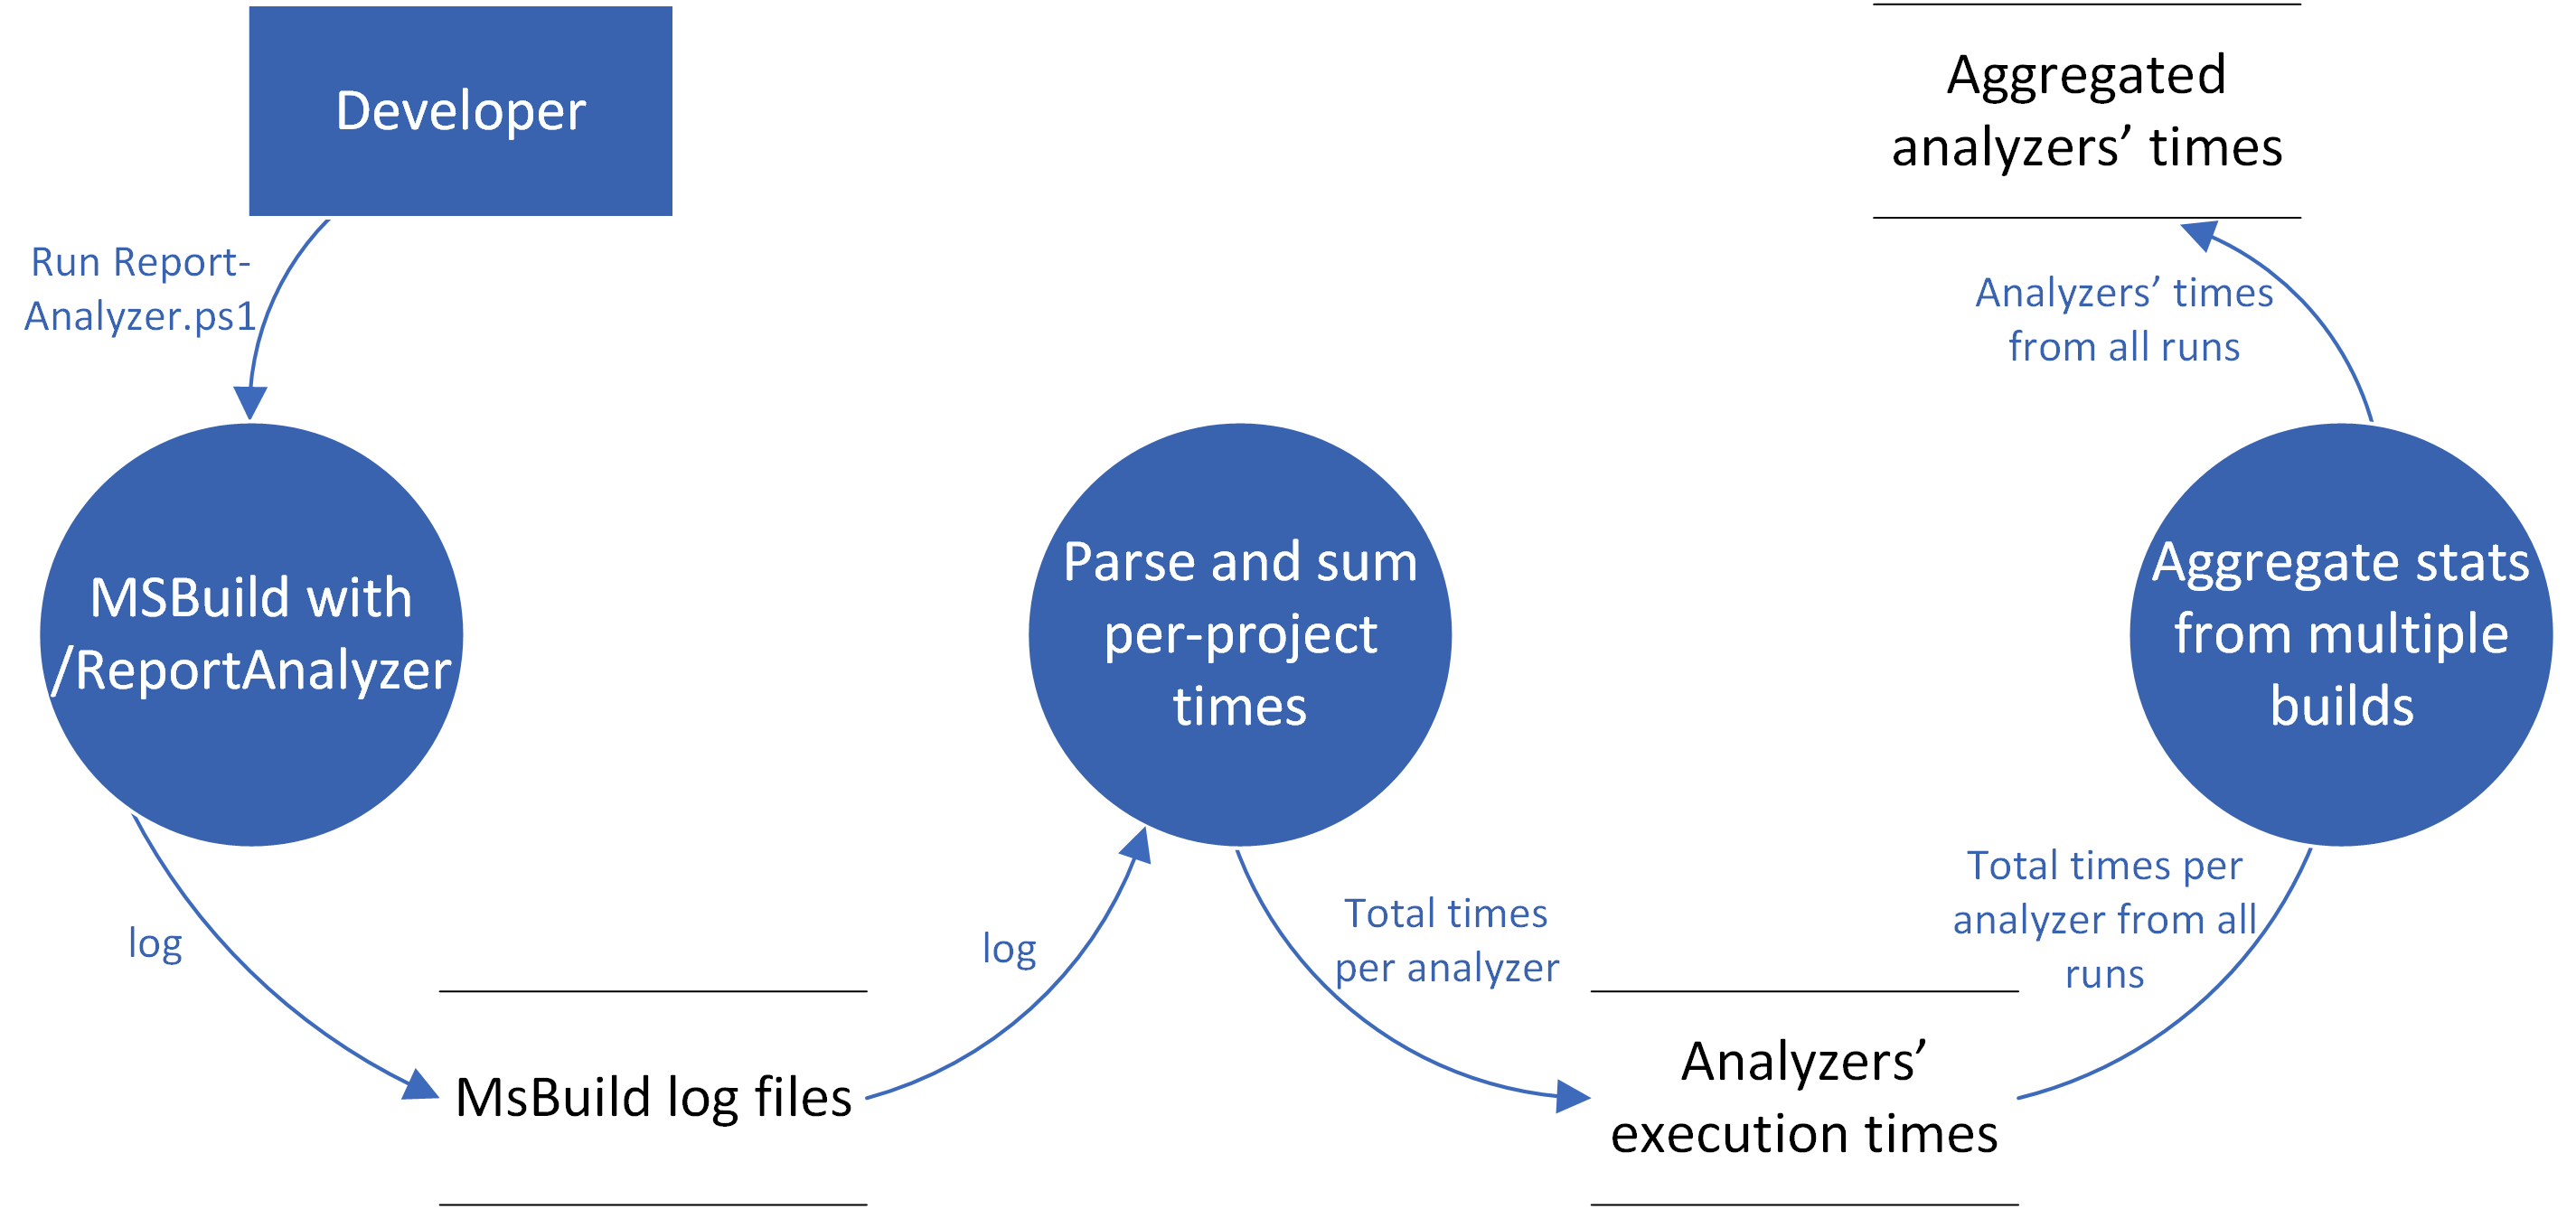
\includegraphics[scale=0.98]{img/uml/report-analyzer-dfd}
		\caption{Data flow diagram for \textit{Report-Analyzer.ps1} script. First two processes are run arbitrary number of times.}
		\label{fig:uml-report-analyzer-dfd}
\end{figure}

\section{Optimizations}
The procedure described in previous section was used to ...

\subsection{System.IO Analyzer}
Most of the optimizations effort was done here...
tell about some limits (EmptyCallback, direct SemanticModelAccess...)
Heuristics applied
final approach

\subsection{Other Optimizations}
Just quickly mention other optimizations 

\subsubsection{\textbf{CMS Base Classes Analyzers}}
symbol vs syntax - perf diftqferences

\subsubsection{\textbf{Syntax Heuristics for Method Invocation Analyzer}}
stats on how much it speeded up relevant analyzers

\subsubsection{\textbf{String Analyzers}}
how not using the generic MethodInvocationAnalyzer influenced the results

\section{BugHunter Analyzers vs Original BugHunter Build Times}
Compare multiple builds w/o BH, old and new versions... Is it significantly slower??

\section{Performance Consideration for Large Solutions}
https://github.com/dotnet/roslyn/wiki/Performance-considerations-for-large-solutions
.. can be used later but so far none of team members complained about worse performance

Why stateful analyzers should not have compilation end actions -- for large solutions it can take more than one minute for the diagnostic to show up in VS... that is not usable at all and cannot be considered as "live" feedback.

\section{Tool Evaluation}
Questionares sent to development team, feedback from senior developers...

% =================================================================
% ============================= CHAPTER 7 =========================
% =================================================================
\chapter{Conclusion}
  - what issue it solved (Equals, Response vs Request.Redirect())
  - what is the~current status of the~project
  - how it helped the~development teams...
  - how to maintain the~tool, 
  - how easy it is to add new analyzers, 

- talk about kentico selling it's source code, so after stabilization, BH could be also available for them as nuget package and aid with the~development practices 
%
%\section{Roslyn as SDK and Its Usage -- Considerations and Remarks}
%Changing versions ... not really well documented
%Only issues on GH provide some insight
%e.g. SkipGeneratedCoOdeAnalysis or RunAnalyzersInParallel - some discussions on GitHub but not clear outcomes, sometimes proposition does not math the~actual implementation and it is generally hard to find some best practices on how to do stuff ad it is still a~pretty young tech... moreover the~examples are not really updated according to new versions of the~API so one struggles with implemeting something on his own only to find a~few weeks later that it was added or it is considered for the~next milestone
%
%many useful things are marked as internal in the~source code and there are many issues on GH to make them public
%
%current version used is v.1.3.X and for this on VS with Update 3 is needed... had to be installed on all build boxes to accomodete BH depoloyment
%
%... version v2 was released after the~implemetnation was finished and it was considered although it was agreed we will not use it as it required VS2017 and nobody is happy about it.. talk about some cons...
%
%(  - ConfigureGeneratedCodeAnalysis - big boost when roslyn API allowed to opt out for analyzer to be run on generated code. Before, heuristics had to be performed by analyzers themselves on every callback
%   https://github.com/dotnet/roslyn/issues/6998
%   https://github.com/dotnet/roslyn/pull/7526)
%
%- problem with Symbol location and disappearing diagnostic 

% =================================================================
% =============================== STUFF ===========================
% =================================================================
	% From template
	\makeatletter\thesis@blocks@clear\makeatother
	\phantomsection %% Print the~index and insert it into the
	\addcontentsline{toc}{chapter}{\indexname} %% table of contents.

	\printindex
    
% =================================================================
% =========================== BIBLIOGRAPHY ========================
% =================================================================
  \printbibliography

% =================================================================
% ============================ APPENDICES =========================
% =================================================================    
\appendix %% Start the~appendices.
\chapter{Source Codes in IS}
\label{appendix:source-codes}
  The main solution with new Roslyn analyzers (BugHunter.sln) consists of 6 projects within 2 folders: TODO - Do leave the~Vsix project there or delete???

TODO - replace with a~screenshot???
\begin{description}
  \item[Analyzers folder] with Roslyn analyzers
  \begin{itemize}
    \item BugHunter.Core
    \item BugHunter.Analyzers
    \item BugHunter.Web.Analyzers
  \end{itemize}
  
  \item[Tests folder] with tests:
  \begin{itemize}
    \item BugHunter.TestUtils
    \item BugHunter.Core.Test
    \item BugHunter.Analyzers.Test
    \item BugHunter.Web.Analyzers.Test
  \end{itemize}
\end{description}

TODO Describe each project.. why 2 for analyzers - nuget distribution

The projects with analyzers use the~categories also for folder structure with each folder containing separate subfolders for analyzers and code fixes respectively.
\chapter{Questionnaires}
TODO...

Sum up the questionnaire results and cite teamleaders' feedback on the tool.

\chapter{Deployment and Versioning}
\label{appendix:deployment}
TODO...
\section{Two NuGet packages with BugHunter Analyzers}
Why, how -- only referr to appendices where this is described

\section{Applying old BH configuration}
what approaches were taken - ruleset file, pragma statements, not installing analzyer nuget at all...

talk about the~old configuration of the~BH, and how this one maps to Roslyn version (suppression pragmas vs supression files, some analyzers look at the~filepath or file extension directly.. some chcecks like SystemIO had to be supressed - level set to none in ruleset file - for files that it did not make sense for... helpers that wrap the~"forbidden" functionality were marked with pragma statements around the~whole class so that it is clearly visible in code)

\chapter{Analyzers' Documentation}
TODO...
same as will the online documentation?

IDs, categories, which nuget, title, description, what for, severity, enabled by default...
\end{document}
